\documentclass[10pt, oneside, titlepage]{ltjarticle}  % bxjsarticleの代わりに
\usepackage[haranoaji]{luatexja-preset}
\usepackage[margin=25truemm]{geometry}
\usepackage{graphicx}
\usepackage{titling}
\usepackage{here}
\usepackage{ascmac}
\usepackage{amsmath}
\usepackage{amssymb}
\usepackage{ulem}
\usepackage{url}
\usepackage{mathtools}
\usepackage{float}
\usepackage{listings,jvlisting}
\usepackage[unicode,bookmarks=true,bookmarksnumbered=true,bookmarksopen=true,colorlinks=true,linkcolor=blue,urlcolor=blue]{hyperref}
\newcommand{\diff}{\mathrm{d}}
\def\qed{\hfill $\Box$}

% Listings Configuration
\lstset{
    basicstyle={\ttfamily},
    identifierstyle={\small},
    commentstyle={\small\itshape},
    keywordstyle={\small\bfseries},
    ndkeywordstyle={\small},
    stringstyle={\small\ttfamily},
    frame={tb},
    breaklines=true,
    columns=[l]{fullflexible},
    numbers=left,
    xrightmargin=0em,
    xleftmargin=3em,
    numberstyle={\scriptsize},
    stepnumber=1,
    numbersep=1em,
    lineskip=-0.5ex
}

% Change "Listings" to "プログラム"
\renewcommand{\lstlistingname}{プログラム}

\title{ \large{2024A・機械情報冬学期演習・自主プロジェクト}\\
\vspace{1cm}
\Huge{卓球ロボット HARIMOTO}}
\author{東京大学工学部機械情報工学科3年 \\
学籍番号: 03-240281 \\
氏名: 椿 道智}

\begin{document}
\begin{titlepage}
  \begin{center}
  \Large{2024A・機械情報冬学期演習・自主プロジェクト}\\
  \vspace{1cm}
  \Huge{卓球ロボット HARIMOTO}\\
  \vspace{1cm}
  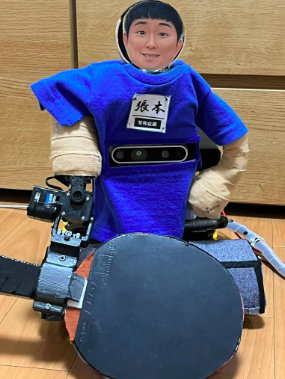
\includegraphics[width=10cm]{figures/HARIMOTO.png}\\
  \vspace{2cm}
  \Large{
  東京大学工学部機械情報工学科3年\\
  学籍番号: 03-240281\\
  氏名: 椿 道智
  }
  \end{center}
\end{titlepage}
\section{概要}
本プロジェクトでは,卓球台上を移動可能な卓球ロボット HARIMOTO(以下,単に「ロボット」という.)を製作した.ロボットは,「プッシュ卓球打ち(=温泉卓球打ち)」「ドライブ打ち」の二種類の打撃方法により,投げた卓球ボールに対して,タイミングを合わせてラケットを振ることができる.単に,打撃制御や画像処理をするだけではなく,ボールが返球された際の「チョレイ」効果音や外装の工夫により,実際の張本選手感(卓球選手感)を出し,ユーザ側が楽しめるようにも工夫した.

ソフトウェア面では,アームの動作(卓球ボールの打撃),D435iによる画像認識(卓球ボールの認識),ボールの着地予測,メカナムホイールの制御,音声再生を行った.機械工学少人数ゼミ(岡田慧教授ゼミ)や知能ロボット演習(機械情報冬学期演習)で学んだeuslisp・ROS noeticを用いてシステムを組んだ.

ハードウェア面では,4自由度アームの設計・製作,ラケットや服,左腕や靴など外装の製作・塗装を行った.

なお,プレゼンでは技術的なことを永遠と喋っていても生産性がないので,わかりやすさ重視で技術的な詳細をあえて省いた.本レポートでは,それを補う意味でも,技術的にこだわった点・細かい工夫などを詳細に記述する(粒度がかなり細かい)ので,興味のないところは適宜読み飛ばしていただきたい.

\section{動機・背景}
私は手術ロボットや医療ロボットに興味があり,特に縫合など針を使った自律的なタスクに関心がある.そのため,学期の初めには縫合ロボットを作ろうと考えていた.しかし,少人数ゼミで縫合に挑戦する機会が得られたため,自主プロジェクトではあえて全く異なるタスクのロボット製作に取り組むことにした.

自主プロジェクトは「何でも作っていい」という貴重な機会であるため,自分の趣味である卓球ロボットを作り,「自分が楽しむ」ことを最優先に考えた.卓球ロボットといえば,従来研究では卓球台の外に大きなパラレルリンクを設置して返球させる手法が主流なのは周知の通りである\cite{omron}.しかし,似たようなものを作ってもオリジナリティがないと思い,本プロジェクトでは,従来の方法とは逆に「卓球台の上で省スペース」「シリアルリンク」の新しい卓球ロボットを制作することを目指した.

\section{コンセプト(実現可能性の根拠)}
卓球選手の戦型には,前陣型(速攻型),中陣型、後陣型の3つがある.それぞれの戦型は,卓球台からの距離に応じて,前陣型は台から0〜1m,中陣型は1〜2m,後陣型は2m以上離れた位置でプレーする.

この中で前陣型は,卓球台に非常に近い位置でプレーするため,ボールが台に着地した直後にラケットで返球する.この戦型が存在するということは,理論的にほとんどのボールを台から離れず,着地直後に返球できることが示唆される.

これを前提に,卓球台上でボールを返球するロボットを作成することが可能だと考えた.ロボットは台上で動きながら,ボールが台に落ちた直後に返球できるため,台から離れずに動きながらボールを処理できるというメリットがある.また,ボールが着地した瞬間に返球するため,ラケットの高さを低く設定できる点もメリットである.

一方,前陣型は速攻型とも呼ばれるように,非常に短い時間でボールに反応しなければならないため,ロボットには素早い画像認識と判断能力,移動能力が求められる.この反応速度が,本プロジェクトの課題の一つとなっている.

\section{システム構成}
ロボットのシステム構成を図\ref{system}に示す.ロボットは,4自由度ロボットアーム・Interl D435i depthカメラ・メカナムホイール・スピーカーから構成される.これらと,ホストコンピュータのmain.l(制御アルゴリズム),画像処理のノード(detect\_ball.launchで起動)をros topicを介して通信する方法でシステムが構成されている.
\begin{figure}[H]
  \centering
  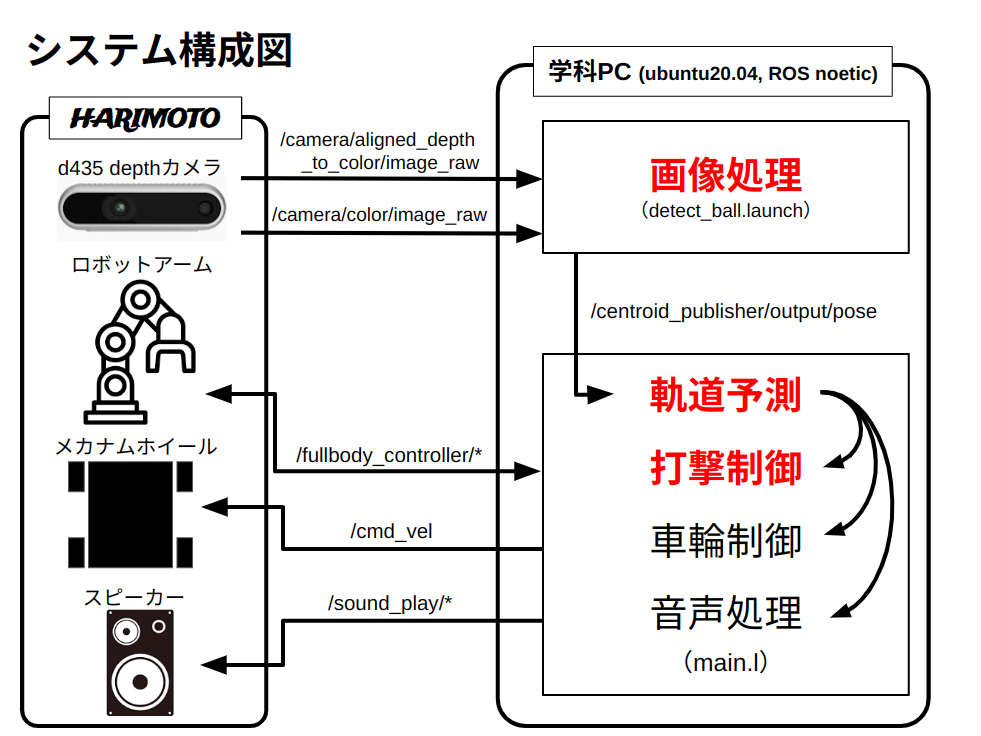
\includegraphics[width=12cm]{figures/system.png}
  \caption{システム構成図}
  \label{system}
\end{figure}
次の5章では図\ref{system}右側の「ソフトウェア」を,6章では図\ref{system}左側のハードウェアや外装について詳しく述べる.

\section{ソフトウェア}
この章ではソフトウェアの実装について述べる.まずは全体を概観したのち,詳しい実装について説明する.
  \subsection{機能の概観}
  ロボットの主要機能は以下の通りである.
  \begin{enumerate}
    \item {\bf 2種類の速度計測}
    \begin{enumerate}
      \item 即時速度
      \item 移動平均速度
    \end{enumerate}
    \item {\bf 着地予測}
    \begin{enumerate}
      \item 着地予想時間
      \item 着地予想位置
      \item 距離ごとに異なる方法
      \begin{enumerate}
        \item 近距離(NEAR)
        \item 中距離(MIDDLE)
        \item 遠距離(FAR)
      \end{enumerate}
    \end{enumerate}
    \item {\bf 着地地点への移動}
    \item {\bf 打撃}
    \begin{enumerate}
      \item プッシュ打ちモード
      \item ドライブ打ちモード
    \end{enumerate}
    \item {\bf 音声}
    \begin{enumerate}
      \item 打撃した際に「チョレイ」と叫ぶ.
      \item サーボに長時間負荷をかけるとモータが焼けるので,一定時間経過後アラームを鳴らす.
    \end{enumerate}
  \end{enumerate}

  以下,これらの機能をどのように実現したか各プログラムとその統合について述べる.概観→詳細の順で説明したほうがわかりやすいので,上層のインテグレーションから説明する

  \subsection{インテグレーション(ROS package HARIMOTO)}
  ロボットをROS noeticで動かすために,卓球ロボットの知能処理プログラムとロボットのモデルなどを1つのROS package "HARIMOTO"としてまとめた.構成は以下の通りである.
  \begin{screen}
  ├── CMakeLists.txt \\
  ├── config \\
  │   ├── HARIMOTO\_servo\_config.yaml \#サーボIDの設定 \\
  │   ├── joint\_names\_HARIMOTO.yaml \#サーボとモデルのジョイントのインタフェース \\
  │   └── mecanum\_drive\_controller.yaml \#メカナム制御の設定 \\
  ├── launch \\
  │   ├── all.launch \#下記のlaunch+sound\_playノード等をまとめて起動する \\
  │   ├── detect\_ball.launch \#ボールの画像認識ノードの起動 \\
  │   ├── mecanum\_drive\_controller.launch \# ros:ridgeback\_controlのノードの起動 \\
  │   └── minimal.launch \#KXR controllerの起動 \\
  ├── meshes \#ロボットモデルのメッシュファイル(STL) \\
  ├── package.xml \#packageの依存関係の定義 \\
  ├── src \\
  │   ├── HARIMOTO-interface.l \#KXR controllerとmainコードのインタフェース \\
  │   ├── HARIMOTO-speak.l \#音声再生のインタフェース  \\
  │   ├── main.l \#メインプログラム  \\
  │   ├── falling-point-estimation \#着地予測の複雑な処理(今回は使わない)  \\
  │   └── scan\_ids \#サーボIDのスキャナ \\ 
  ├── file \#「音声再生」に用いるファイル群 \\
  │   ├── start.mp3 \\
  │   ├── chorei.mp3 \\
  │   └── warn.mp3 \\
  └── urdf \\
     └── HARIMOTO.urdf \#ロボットモデル
  \end{screen}
  以降では,上記のファイルが実際にどのような働きをするのかに注目しながら,ソフトウェアの実装を述べる.
  \subsection{ロボットモデルとハードウェアインタフェース}
    \subsubsection{ロボットモデルの作成}
    Solidworks(CADソフト)でアームの設計をした後,ROS用のロボットモデルとして"HARIMOTO.urdf"と関連メッシュファイルをurdf-converterで出力した.この自動で出力したURDF(ロボットモデルファイル)には,アームのjoint情報とlink情報しか記述されていないので,さらに,D435i Depthカメラの座標(Camera\_link)の情報や,メカナムホイールのJOINT, LINKの情報,ロボットの胴体のLINKの情報を手作業で変更した(このCUIでURDFを書き換える作業がかなり大変だった).次いで,"servo\_config.yaml"や"joint\_name.yaml"でサーボID情報やURDFのJOINT名とサーボIDの対応付けを行った.

    \subsubsection{ロボットモデルとeuslispとのインタフェール}
    "src/HARIMOTO-interface.l"を,演習の"jedy-interface.l"を真似しつつ,不要なメソッドなどを削除することで,記述した.これにより,euslispで"(send ri :<method>)”によりロボットの行動計画を行うことが可能となった.
    \subsubsection{ハードウェアインタフェース}
    コンピュータとロボット(モータ)とのハードウェアインタフェースについては,jedyの演習で用いた"KXR\_controller"というpackageを用いた.そのKXR\_controllerのノードを起動するためにjedy同様"minimal.launch"を記述した.これを立ち上げることで,euslispで書いたコードが実機で動くようになる.

    \subsection{打撃〜アームの行動計画〜}
    本ロボットでは,4自由度アームの軌道生成によって,打撃を実現している.卓球の場合は,ラケットの向き(=エンドエフェクタの姿勢)が重要となる.一方,位置と姿勢を一意に指定するためには6自由度が必要でinverse kinematicsが解けない.\footnote{卓球はラケット平面が決まればその面にそってラケットを滑らせるだけなので,4自由度で足りるのではないかという仮説に基づいて,コストカットのために4自由度にしたが,プログラムの視点で見ればIKが解けないのは絶望的に面倒なことをしたと反省している.}そこで今回は,実験的にアームの軌道を求めた.
    \begin{enumerate}
      \item サーボオフにする
      \item ロボットのラケットを手で持って打球時の軌跡を描く
      \item その時のサーボモータのangleを取得する
    \end{enumerate}
    の手続きで取得したjoint-angleの値ををそのまま再生しても,重力の影響で思っていた軌道よりもたるんでしまう.そこで,その分のオフセットを入れれば一通り打撃することができる.

    次に,高いボール・低いボールに対応できるように,高さを引数にできるように改良した.根本の関節(肩の関節)を高さによって変え,それによってラケットの面の向きがわかる分を他の関節で調整するようにJOINT軌道を設計した.完成した関数は,以下の通りである.なめらかな動きを実現するために. *ri*のメンバ関数である:angle-vector-sequenceを用いた.

    さらに,各アクチュエータの速度は遅いながら,全体として速い軌道を実現するために,落下方向に降るときに「{\bf 重力}」を利用したり,前方向に降るときに「{\bf 足回り}」を一緒に前に動かすことで,打球時の一瞬にロボットの運動ポテンシャルを最大限発揮できるように工夫して動作を設計している.この部分の軌道設計はかなり苦労した.以下に実際のプッシュ関数の中身を示す.
    \begin{lstlisting}[basicstyle=\ttfamily]
      (defun push-hit(x) ;;引数xには高さの定数倍が入力される
        (let  (p1 *basic-pose-l*) ;; 初期姿勢
              ;; 実験的に求めつつも,高さ引数分の補正を行っている.
              (p2 (float-vector (+ 2 x) 20 10 (+ 30 x)))
              (p3 (float-vector (+ -3 x) 10 10 (+ 20 x)))
              (p4 (float-vector (+ -7 x) 0 10 (+ 10 x)))
              (p5 (float-vector (+ -13 x) -5 15 (+ -0 x)))
              (p6 (float-vector (+ -20 x) -10 20 (+ -15 x)))
              (p7 (float-vector (+ -35 x) -20 25 (+ -35 x)))
              (tm 25))
          ;; 
          (send *ri* :send-cmd-vel-raw 0.01 0 0)
          (send *ri* :angle-vector-sequence 
                (list p1 p2 p3 p4 p5 p6 p7 p1) 
                (list tm tm tm tm tm tm tm 2000)
                :default-controller 0.001
                :min-time 0.00001
                :minjerk-interpolation nil)
          (chorei)
          (ros::duration-sleep 0.5)
          (send *ri* :send-cmd-vel-raw -0.01 0 0)
          (send *irtviewer* :draw-objects))
      \end{lstlisting}
      他にも,ドライブモードを実装したが,オフセットのパラメタ調整が発表までに間に合わなかった.

  \subsection{ボール位置の検出}
  Intel RealSense Depth Camera D435iを用いたボールの中心位置の取得するプログラムついて説明する.

  はじめは,少人数ゼミや演習で試したようにHSIカラーフィルタでフィルタリングした点群のユークリッド距離クラスタリングをして,そのクラスタの中心位置を取得していた\cite{detect2}.しかし,このシステム構成だと,処理が遅く,ボールを見逃してしまい,卓球ボールの認識システムとして機能しなかった.
  そこで,矢野倉先生にご相談したところ,クラスタリングの処理が重いということだったので,「HIVフィルター」でマスクした点群の重心(centroi)を取得することを提案していただき\cite{detect1},発表時点では,そのようなシステム構成とした.具体的には,
  \begin{enumerate}
  \item colorのフレームに対してカラーフィルタを作る \\
  opencv\_apps/hsv\_color\_filter
  \item colorフレームのフィルタをdepthフレームに適用できる形にする \\
  jsk\_perception/depth\_image\_filter
  \item depthフレームを2.のフィルタでマスクする \\
  jsk\_perception/ApplyMaskImage
  \item フィルタ後のdepth画像の重心を取得してpublishする \\
  jsk\_pcl\_utils/CentroidPublisher
  \end{enumerate}
  のノードを順に実行している.

  上記のノードの構成についてはノードを起動するための"detect\_ball.launch"に記述してある(\url{https://github.com/Michi-Tsubaki/ping-pong-robot/blob/main/src/HARIMOTO/launch/detect_ball.launch}, コメントアウトが旧ver).

  なお,DepathカメラD435iの起動には,realsense-ros packageを用いて,roslaunch realsense2\_camera rs\_camera.launch で起動している.rs\_camera.launchを書き換えることで,ColorとDepthのフレームレートを変更でき,今回は,ハードウェア上の限界である60fpsに設定した.\cite{detect3}
  はじめはusb2.0を使用しており,最大フレームレートが15fpsに留まっていたが,usb3.0に変えたことにより,最大フレームレートが60fpsに上がった(こういうハードウェア上の制約も勉強になった).
  \subsection{着地予測}
    \subsubsection{速度計測}
    ボールの着地予測をするために,まずはボールの速度を知る必要がある.速度は,その瞬間の速度(即時)速度
    \[v(t)=\Bigl[\frac{x(t)-x(t-1), y(t)-y(t-1), z(t)-z(t-1)}{dt}\Bigl]^\top\]
    と,3フレーム分の速度が連続で存在したときに,その移動平均を返す.
    \[\hat{v}(t)=[\frac{v(t)+v(t-1)+v(t-2)}{3}~~\mbox{, if } v(t) , v(t-1) \mbox{ and } v(t-2) \mbox{ exist.}]\]
    移動平均を取ることは,ノイズの影響が小さくなる(ローパスフィルタ)一方で,速度情報が遅れてしまったり,速度が連続で取得できなかった場合は無効となる(出力されない)ので注意が必要である.

    \subsubsection{着地予想時間}
    ロボットの着地予想時間は,$z$方向(ロボットの正面方向)のロボットの位置に依存するので,ロボットが打撃できる空間の位置($z_0$)に到達するまでの時間を計測する.
    \[\mbox{Estimated Time} = T = \frac{z(t)-z_0}{v_z(t)}\]
    この式の$v_z(t)$に$v(t)$の$z$成分を用いるか,$\hat{v}(t)$の$z$成分を用いるかは,ボールの距離$z(t)$がロボットに近いか遠いかで決める.

    ボールの位置によって,空間を
    \begin{enumerate}
    \item 近距離 〜 25 cm
    \item 中距離 25 cm 〜 60 cm
    \item 遠距離 60 cm 〜
    \end{enumerate}
    に分け,中距離では$v(t)$を使い,遠距離では$\hat{v}(t)$を用いる.(近距離では予測をせずに即時返球する.)

    \subsubsection{着地予想位置}
    着地予想位置については,単純に,
    \[\mbox{Estimated Point} = {\bf x} = [x(t)+v_x(t)\times T, y(t)+v_y(t)\times T, z_0]^\top\]
    として計算した.二次関数フィッティングも試みたが,卓球ボールがマグヌス効果で二次関数を描かないせいか,単純にボールの軌跡がほぼ直線だからかは考察していないが,着地予想位置の精度がでなかったので,最終的には単純な線形モデルに回帰することになった.

    ボールのz方向の速度が正のとき($v_z>0$)はボールが離れていっているので,着地予測をせず,また,ボールの速度がとても大きいときとても小さいときは,ノイズと判断して,空振りを防ぐため,着地予測を行わないようにした.他にも,予測モデルが線形で情報が不十分な分は,予測に条件を課すことで,カバーしている.

    着地予想位置については,着地予想時間と一緒にros topicとしてPublishするようにした.これにより,Rvizで着地予想位置を描画できる.メッセージの型には,geometry\_msgsのPoseを用いた.着地予測時間をorientation(クオータニオン)の$w$に入れた

  \subsection{メカナムホイール制御}
  メカナムホイールの制御プログラムについて説明する.メカナムホイールは,ROS ControlのRidgeback Controllerを用いることで,左右・前後・斜め移動といったメカナム特有の動きをすることができる\cite{mecanum}.mecanum\_drive\_controller.launchでこのpackageのノードを起動した.あわせて,"HARIMOTO-interface.l"でcmd\_velトピックとその動きを接続するインタフェースを作ってあげることで,euslispで(send *ri* :send-cmd-vel-raw x y rot)と送るだけで,cmd\_velにメッセージが送られロボットの足回りを動かせるようになった.

  また,移動用のサブルーチンとして,基準値よりも左にいるか右にいるか,前にいるか後ろにいるかによって,逐次cmd\_velを送信する「move\_follow」関数と,指定した相対座標に移動する「move\_to」関数を実装した.
  \begin{enumerate}
    \item move\_follow \\
      ロボットが返球に対応できる範囲(sweet\_spot)に対して,逐次更新されるボールの着地予測地点が右にあるか左にあるか,前にあるか後ろにあるかによって,逐次ロボットが動くことを目的としたサブルーチン.
      
    \item move\_to \\
      camera\_link座標系(カメラに固定された座標)からの相対座標で計算されたボールの着地予想着地地点に直接移動することが可能.
  \end{enumerate}

  発表会時点では,move\_follow関数を用いて着地予測地点に移動していたので,移動できる範囲が左右前後10cmくらいに限られていたが,着地予測の精度が高くにあれば,move\_to関数を使ってより広い範囲で移動できるはずだと考えている(スピードがあまり出ないので,当然広々動き回れるわけではない.)

  \subsection{音声再生}
  ここでは,音声に関する実装について説明する.少人数ゼミでPR2ロボットを扱った際に,PR2に会話をさせるインタフェースとして,"speak.l"が存在した\cite{sound}.このソースコードを読むと,ROSのsound\_playパッケージとeuslipsのソースコードのインタフェースになっていることが分かったのでそれを活用した.

  (send *ri* :sound-play \#P"<mp3 fileのpath>")

  とすれば,MP3の音声ファイルを再生することができる.今回は,ユーザが楽しむという観点,サーボモータに長時間負荷をかけ続けてモータが焼けるのを防ぐ観点から
  \begin{enumerate}
    \item 打撃するたびに「チョレイ」と張本のように叫ぶ.
    \item 起動するときに「お相手しましょう!」と元気よく叫ぶ.
    \item プログラム開始後2分後と5分後に「肩が疲れたよ」とアラートを発する.
  \end{enumerate}
  の3種類の音声再生を実装した.
  \subsection{メインプログラムの流れ}
  5.4〜5.7で説明したメインのプログラムは,単純化すれば,図\ref{flow}フローチャートのような流れになっている.
  \begin{figure}[H]
    \centering
    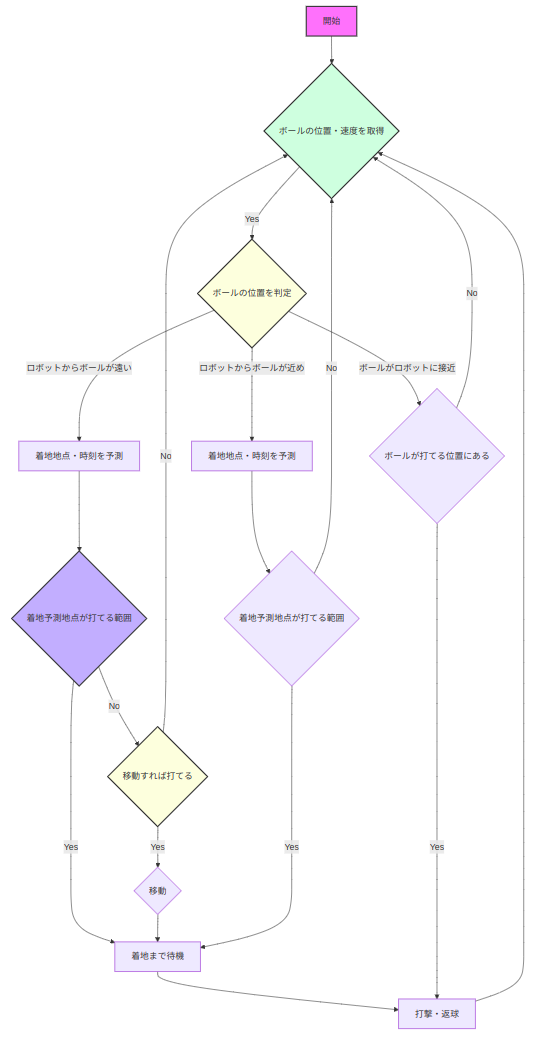
\includegraphics[width=11cm]{figures/flow.png}
    \caption{メインプログラムのフローチャート}
    \label{flow}
  \end{figure}
  以上が,ロボットのソフトウェアの実装である.
\section{ロボットモデル・ハードウェア・メカニクス}
  \subsection{アームの設計・製作}
  KRS-3304R2 ICSサーボモータ(赤サーボ)×1つ,KRS-3302 ICSサーボモータ(青サーボ)×3つ,近藤科学のKXRシリーズのパーツ,自作パー(図\ref{armparts})を用いて,卓球用の4自由度ロボットアーム(図\ref{arm})を設計した.自作パーツはメカのデザイン工房のAdventure 5M(3Dプリンタ)で製作した.材質はPLAである.jedyの7自由度アームをベースにしつつ,卓球に不要な自由度を削除した.

  根本の自由度で高さ(大体の位置)を定め,残りの3自由度でラケットの姿勢(RPY)を指定する.水平平面の2自由度は,足回りで指定できるので,アームでは姿勢と,高さが指定できれば良いという考えに基づいて設計している.
  \begin{figure}[H]
    \centering
    \begin{minipage}{0.48\textwidth}
      \centering
      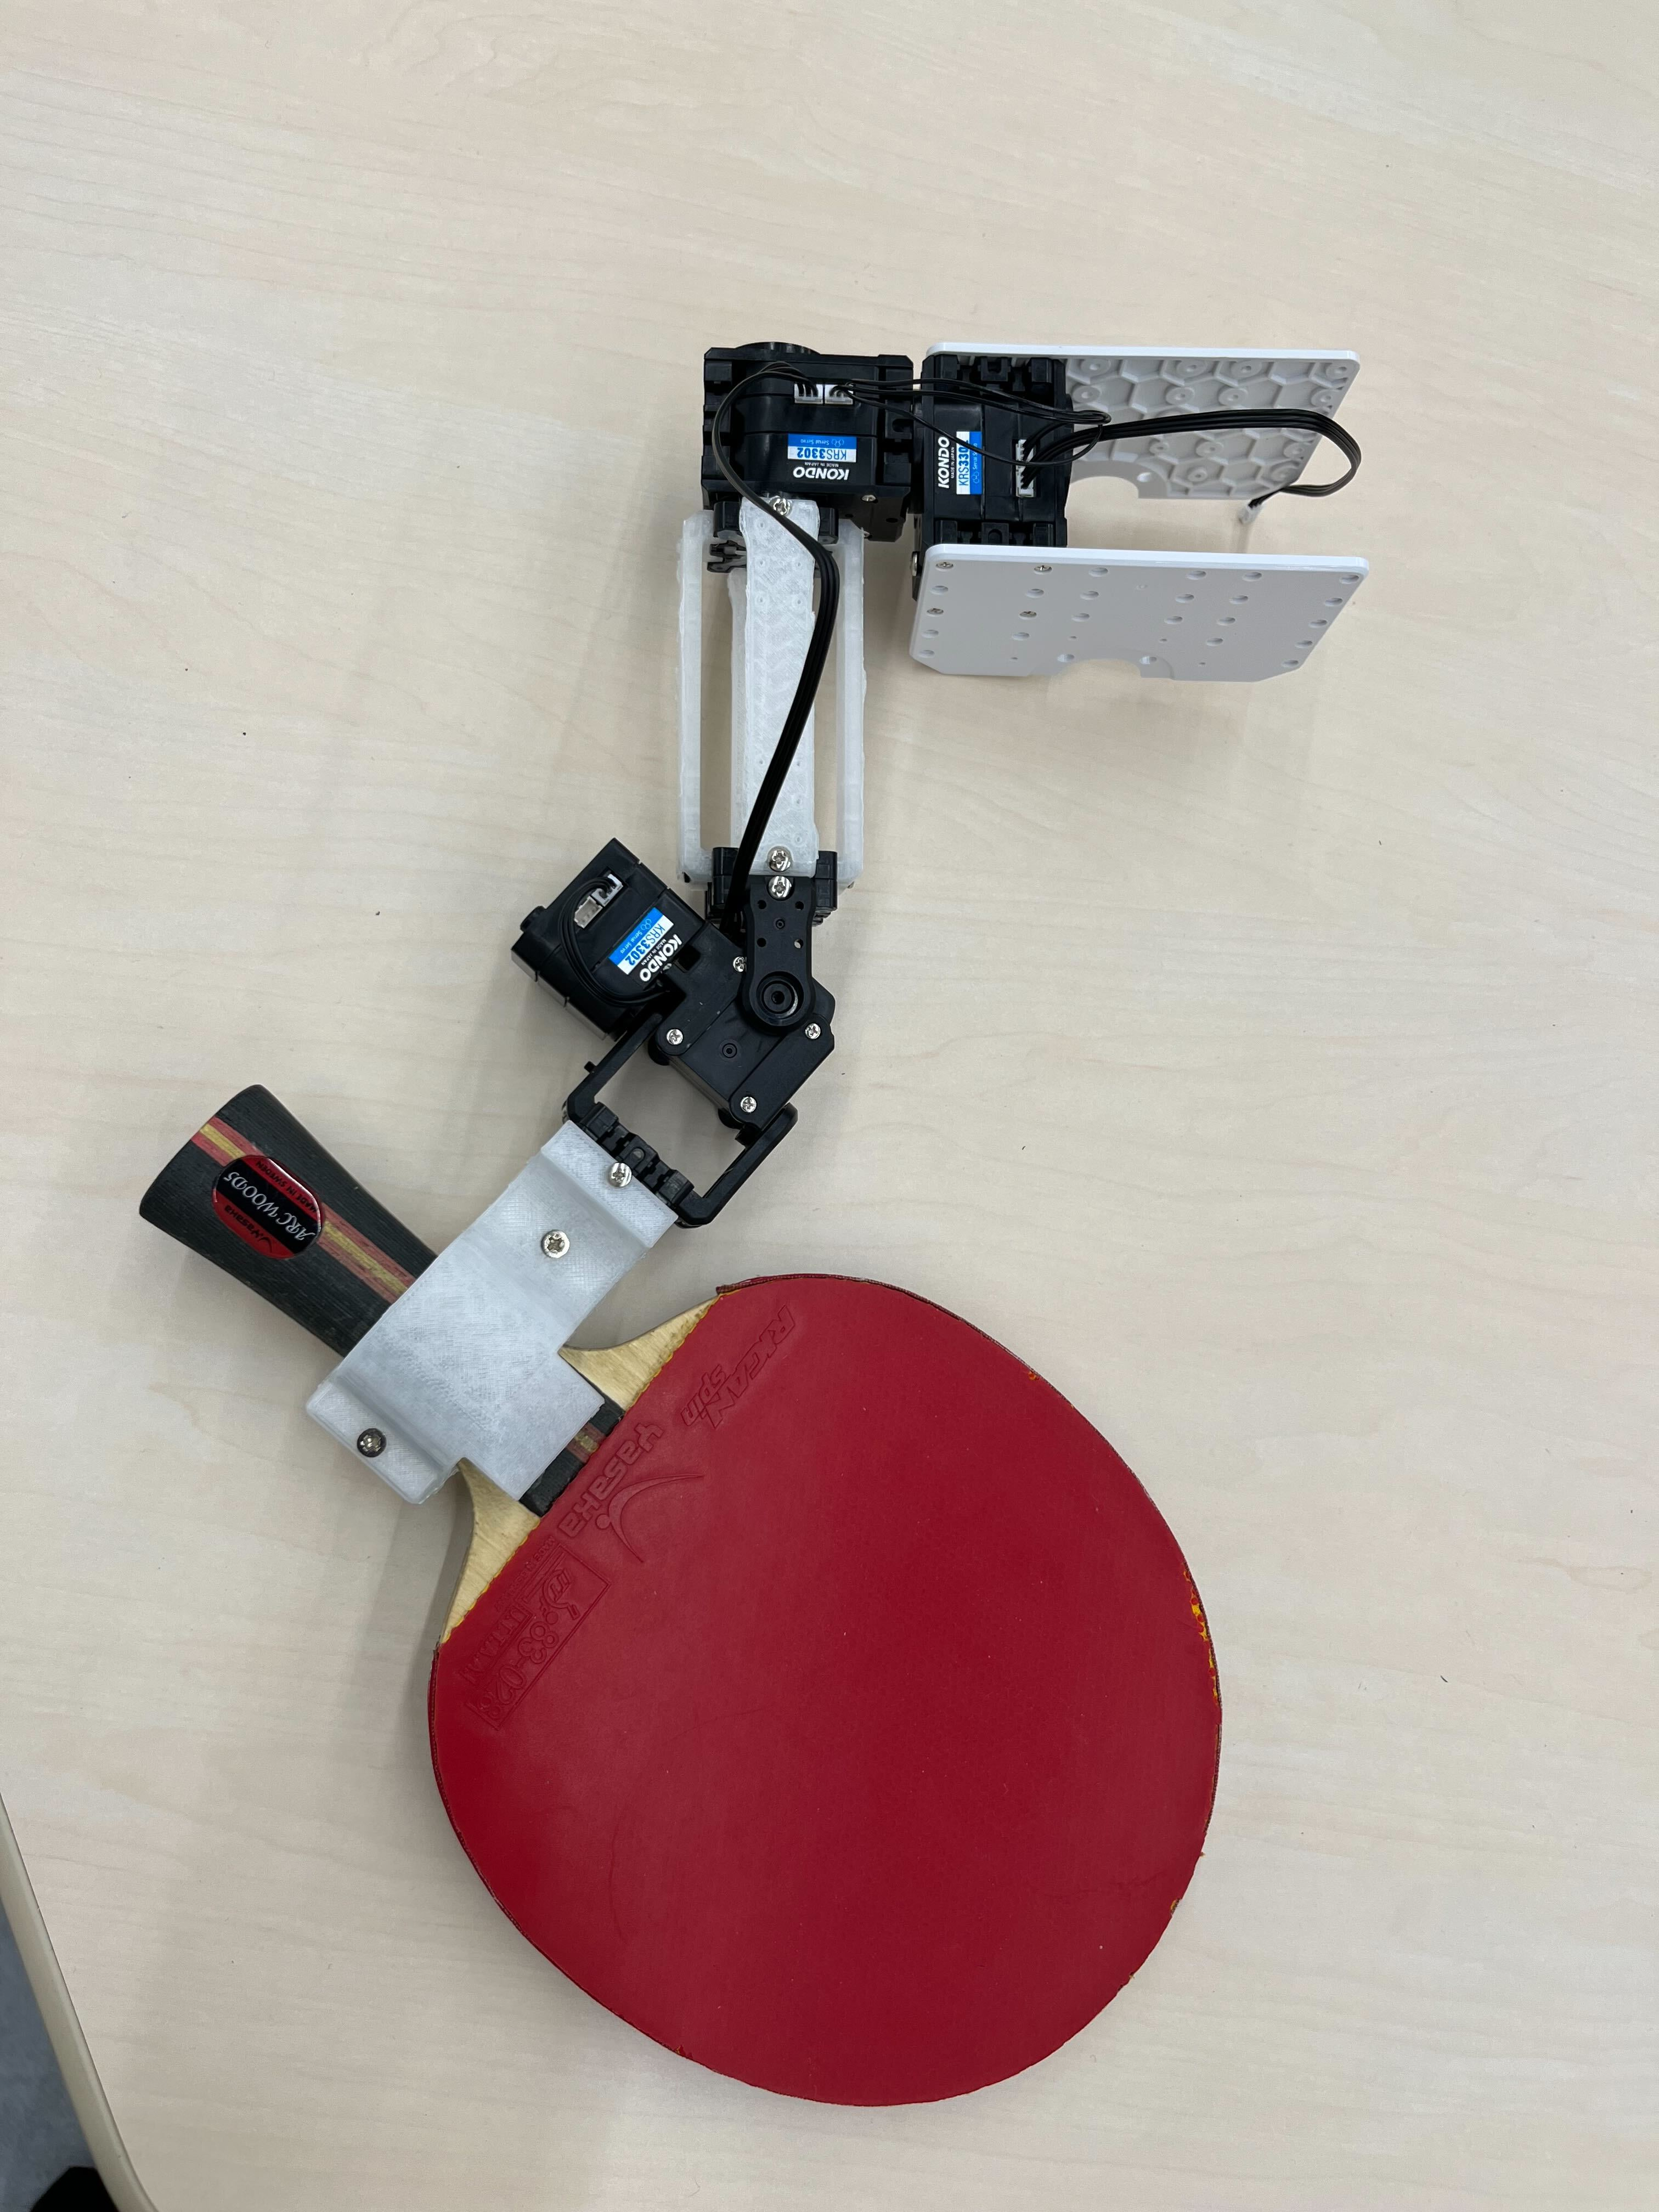
\includegraphics[width=\textwidth]{figures/arm.jpg}
      \caption{4自由度アーム}
      \label{arm}
    \end{minipage}
    \hfill
    \begin{minipage}{0.48\textwidth}
      \centering
      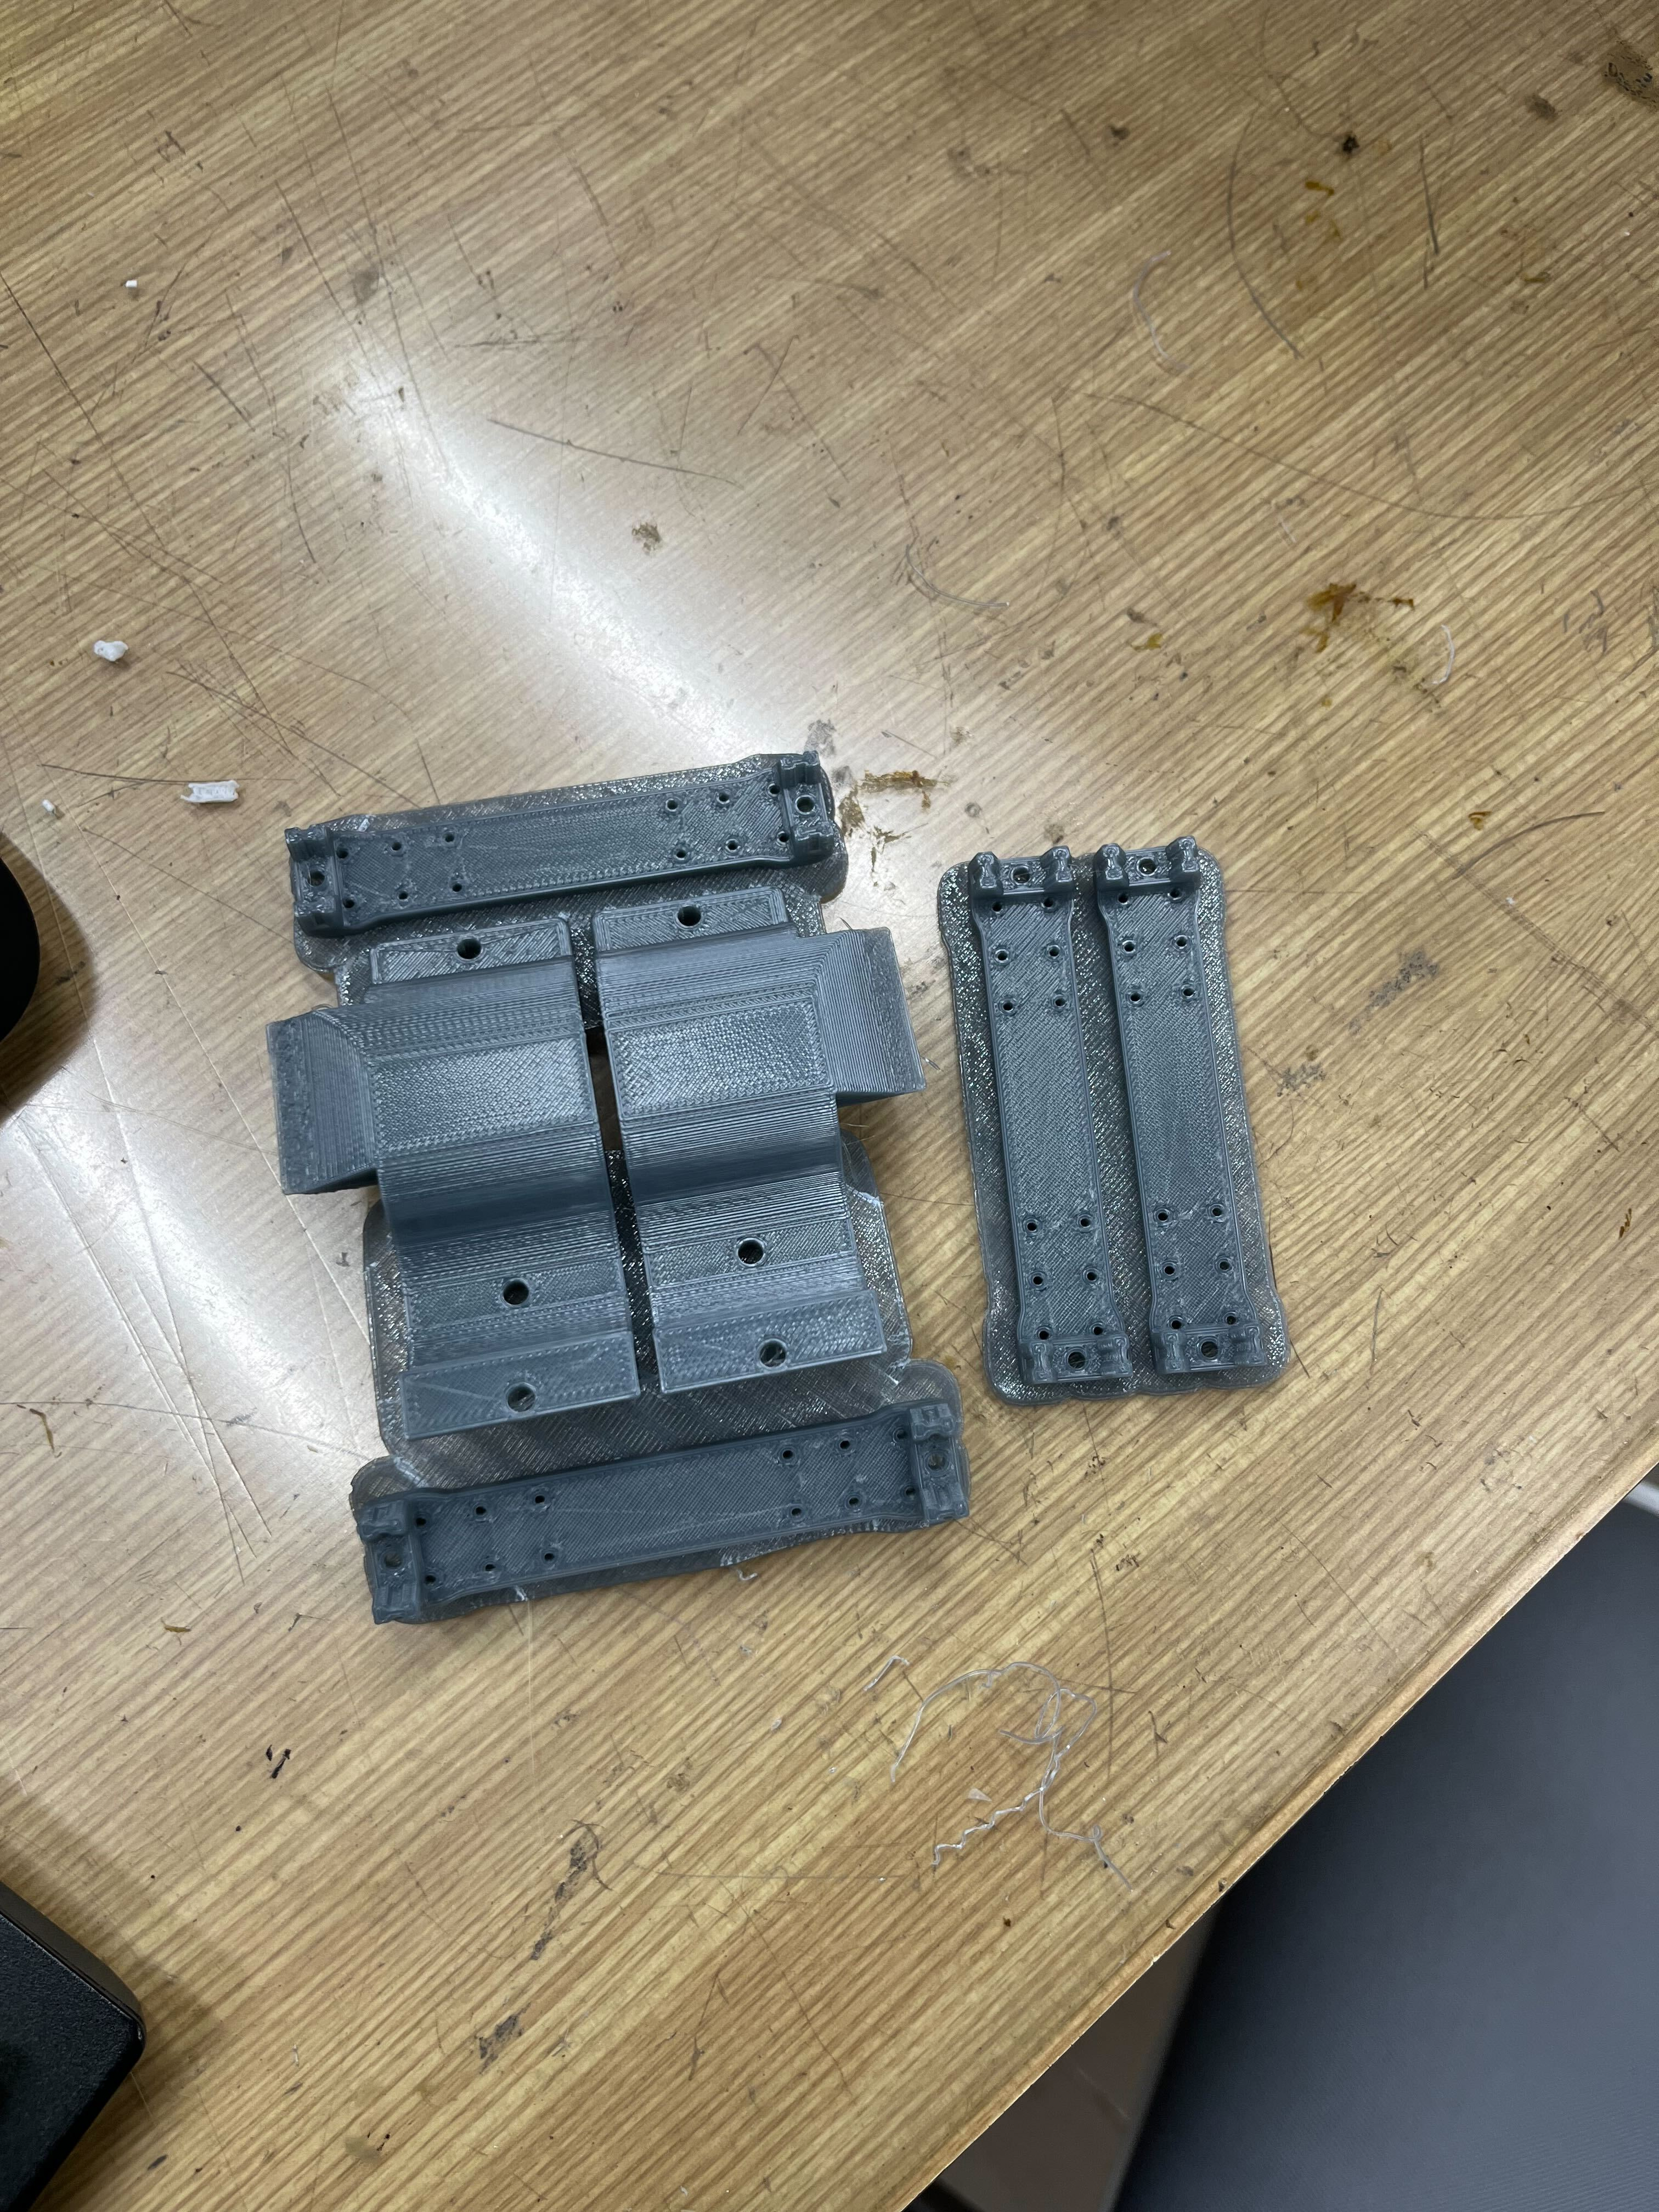
\includegraphics[width=\textwidth]{figures/armparts.jpg}
      \caption{アーム用の自作パーツ}
      \label{armparts}
    \end{minipage}
  \end{figure}

  \subsection{ロボット本体(筐体と車輪のベース)}
  ロボットの筐体(図\ref{body1},図\ref{body2})と,ホイール用のモータを接合するベース板を設計し,メカのデザイン工房のAdventure 5M(3Dプリンタ)で製作した.筐体とベースは一体成型ではなく,別々で製作し,六角ネジで固定している(図\ref{body3}).後に様々な装置をロボットに搭載する可能性を考慮して,ベースいたにはホイール用モータの固定用以外にも多数の穴を開けた.この穴は,実際に,電源装置や靴,スピーカ,おもり(ロボットが軽く車輪が浮いてしまったため,500gの「ホゴオモリ」で重くした)などの設置に役に立った.ベース板の大きな長方形の穴は,モータやカメラのケーブルを通すための穴である.図\ref{body4}のように,青サーボとベース板がネジで接合される.
  \begin{figure}[H]
    \centering
    \begin{minipage}{0.48\textwidth}
      \centering
      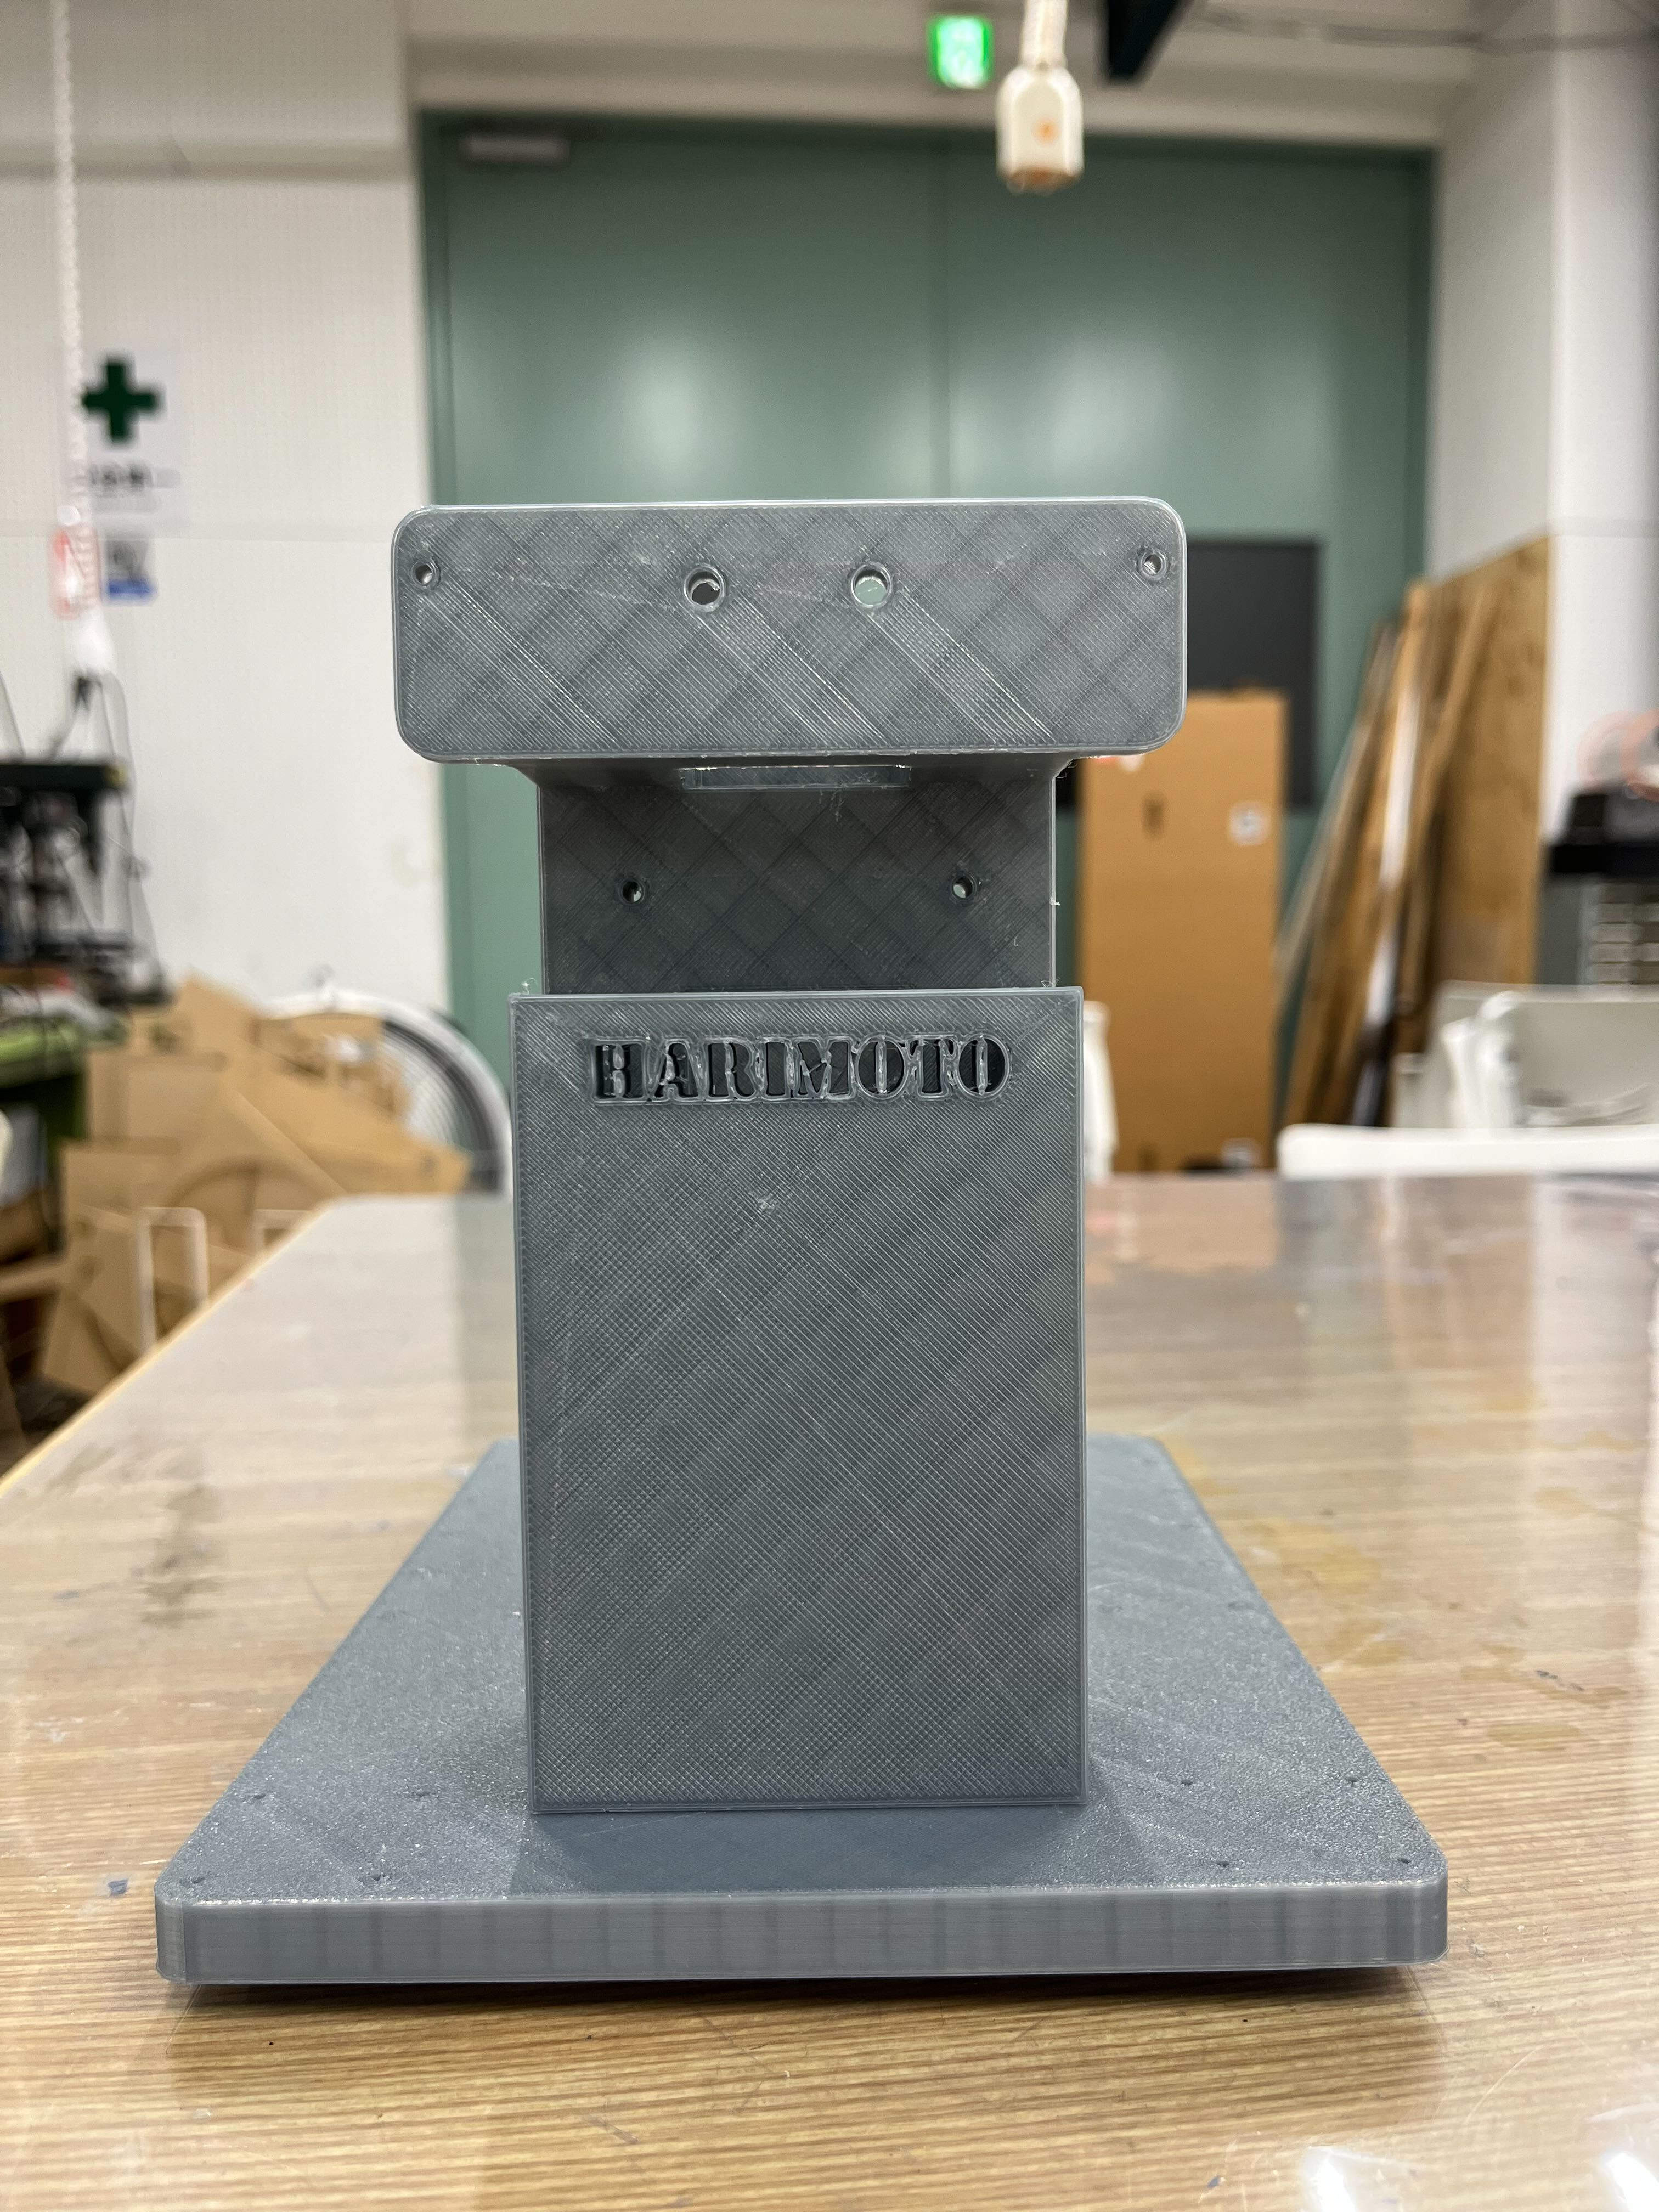
\includegraphics[width=\textwidth]{figures/body1.jpg}
      \caption{筐体(正面)}
      \label{body1}
    \end{minipage}
    \hfill
    \begin{minipage}{0.48\textwidth}
      \centering
      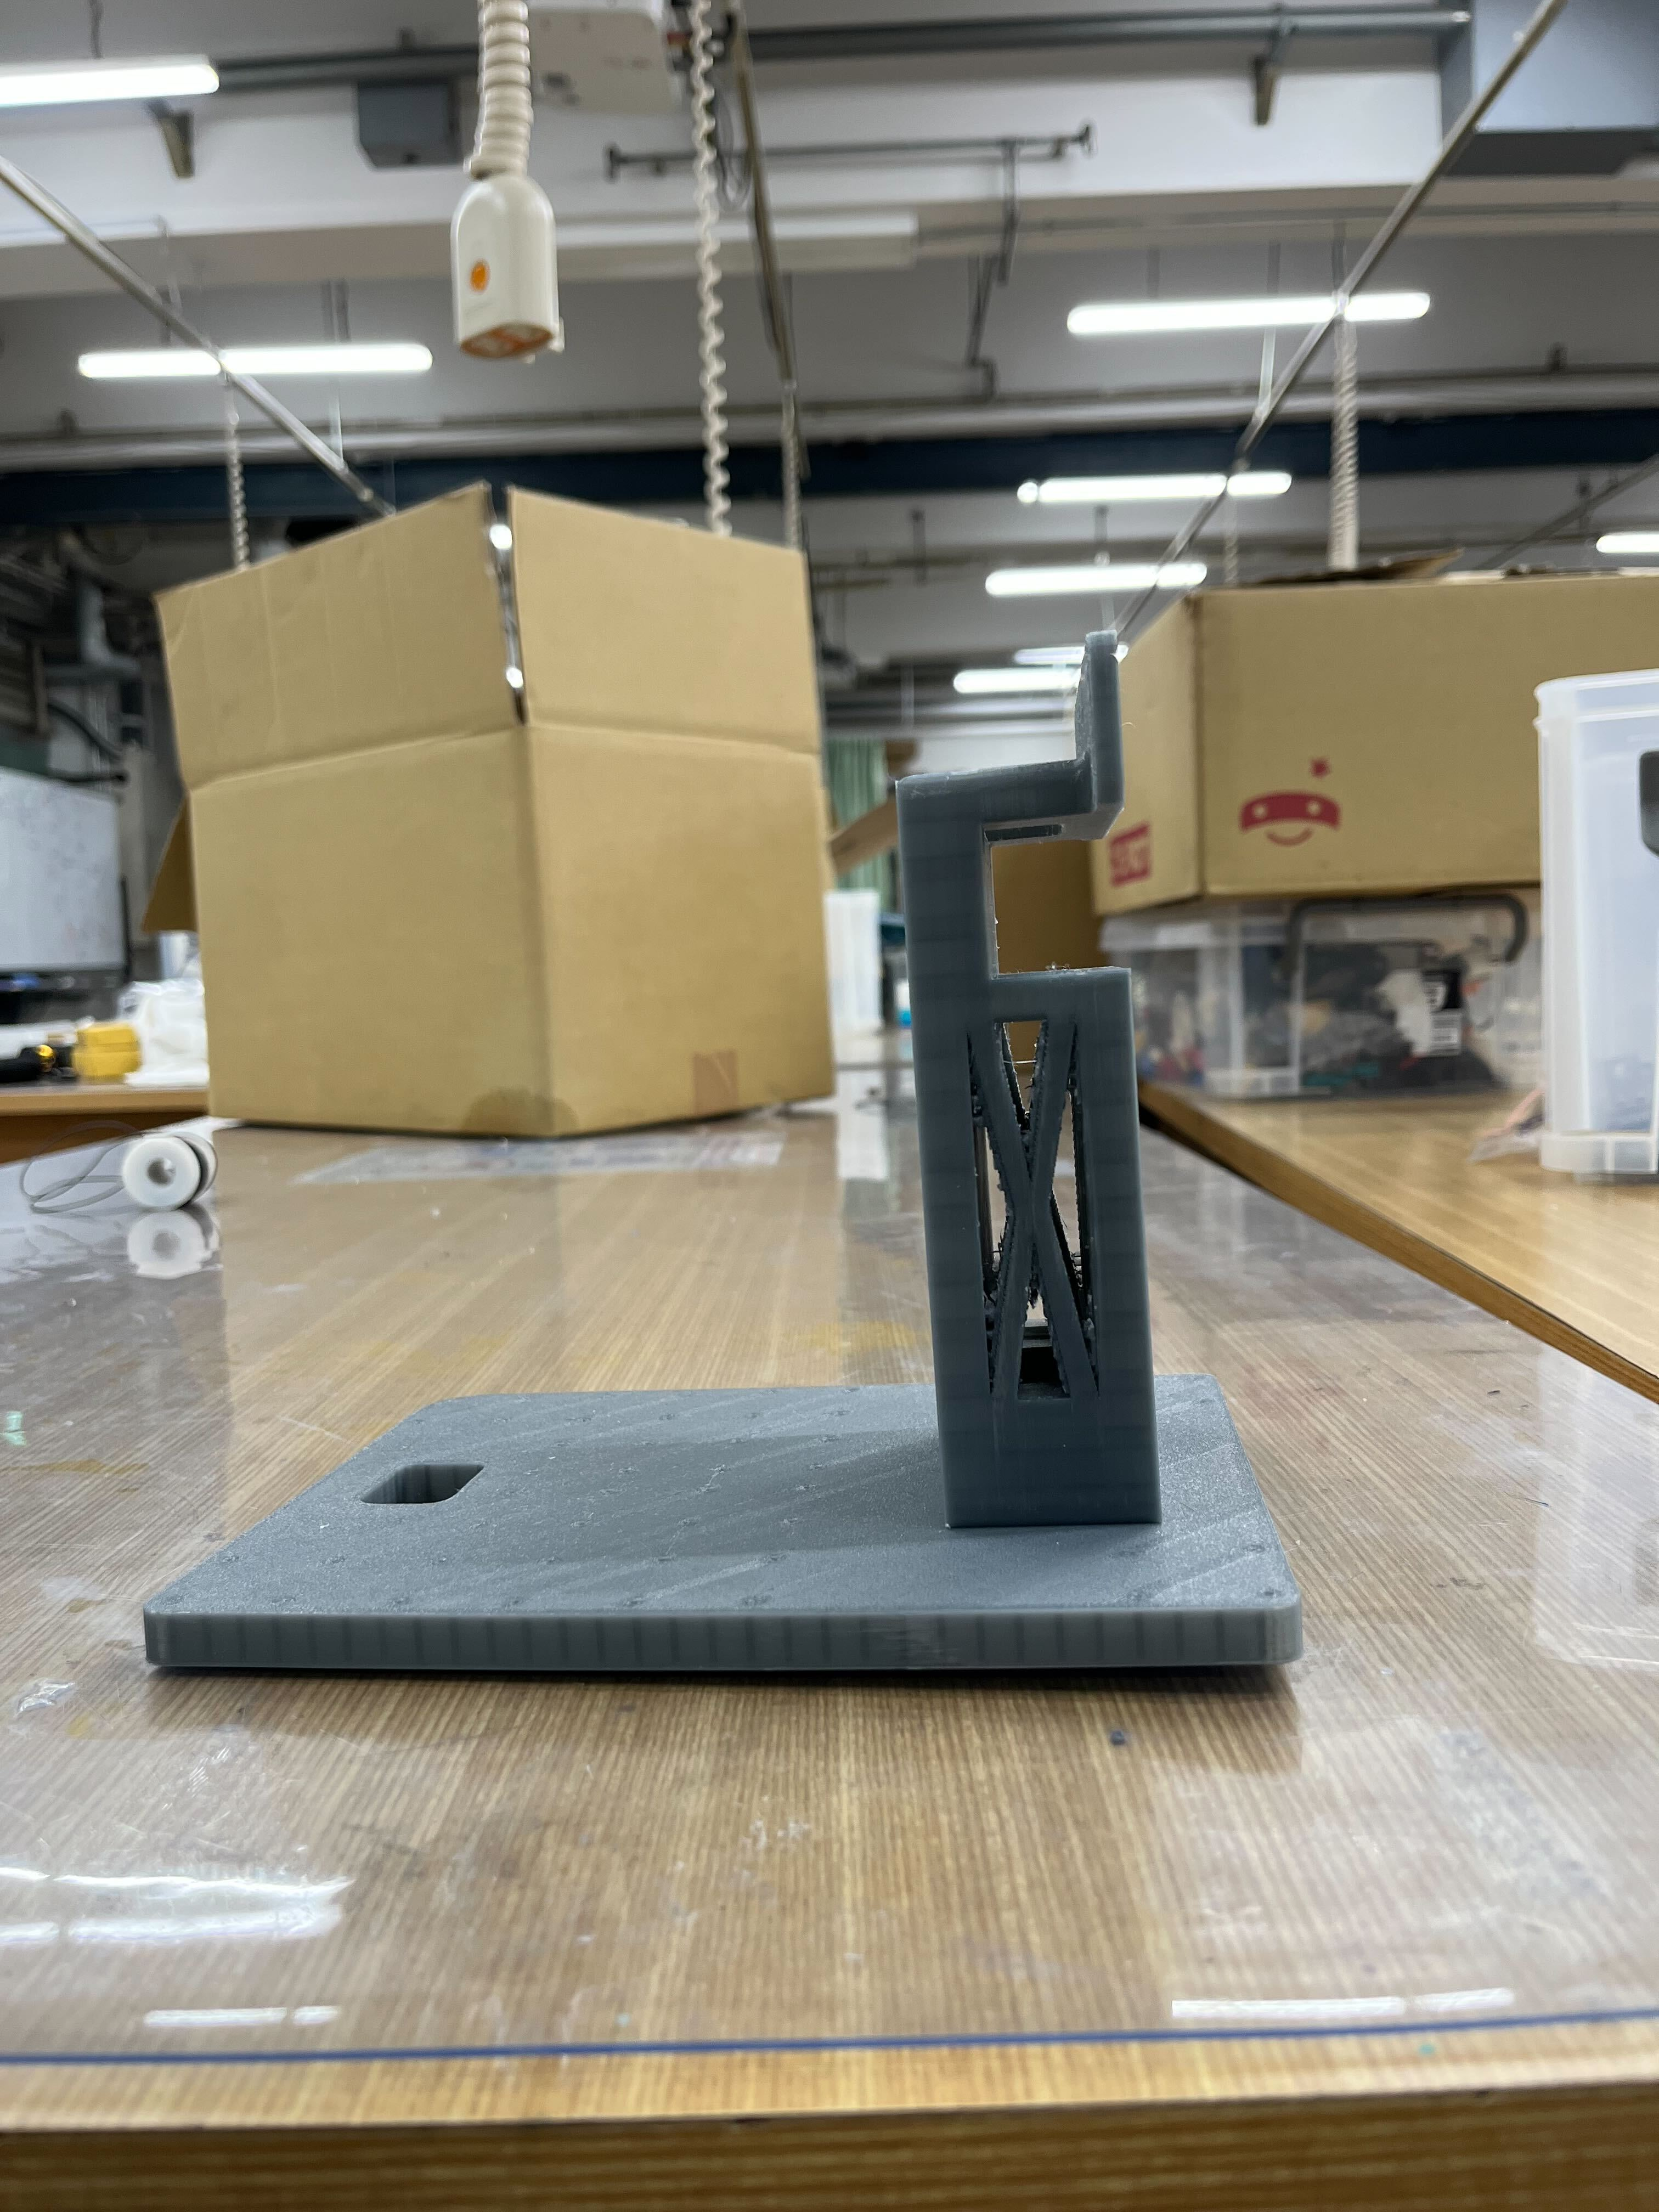
\includegraphics[width=\textwidth]{figures/body2.jpg}
      \caption{筐体(側面)}
      \label{body2}
    \end{minipage}
  \end{figure}
  \begin{figure}[H]
    \centering
    \begin{minipage}{0.48\textwidth}
      \centering
      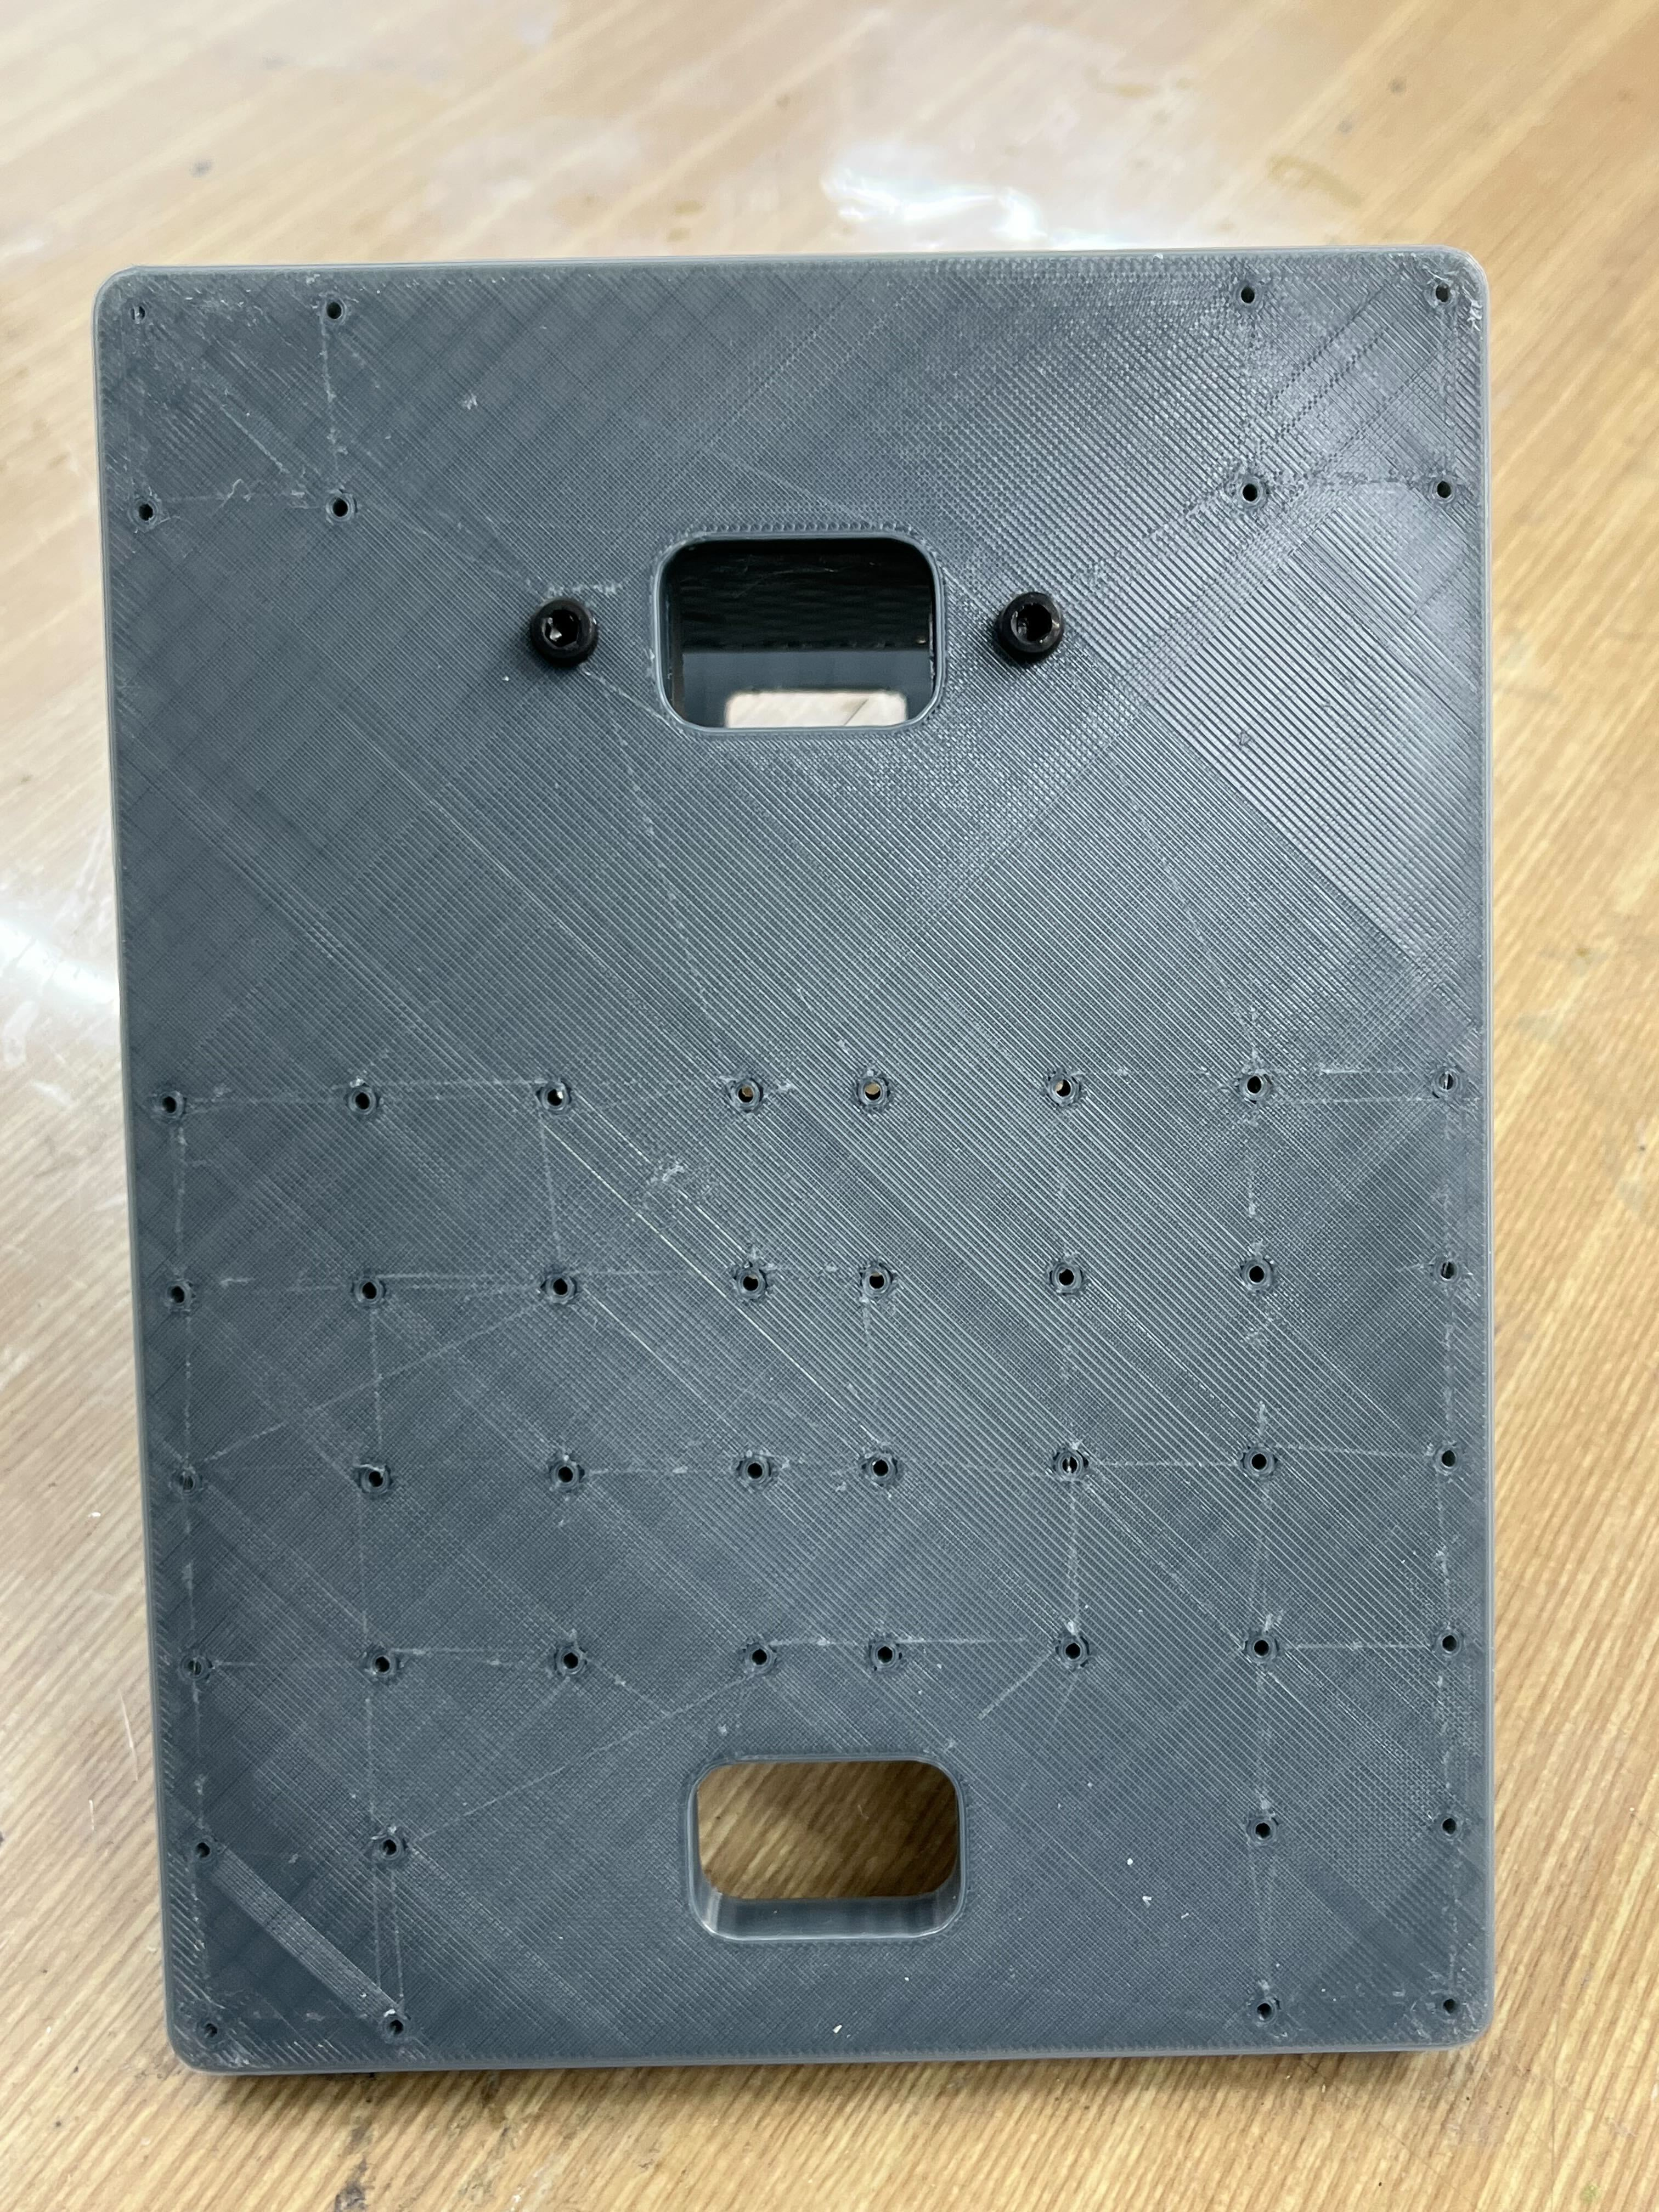
\includegraphics[width=\textwidth]{figures/body3.jpg}
      \caption{ベース板(下から)}
      \label{body3}
    \end{minipage}
    \hfill
    \begin{minipage}{0.48\textwidth}
      \centering
      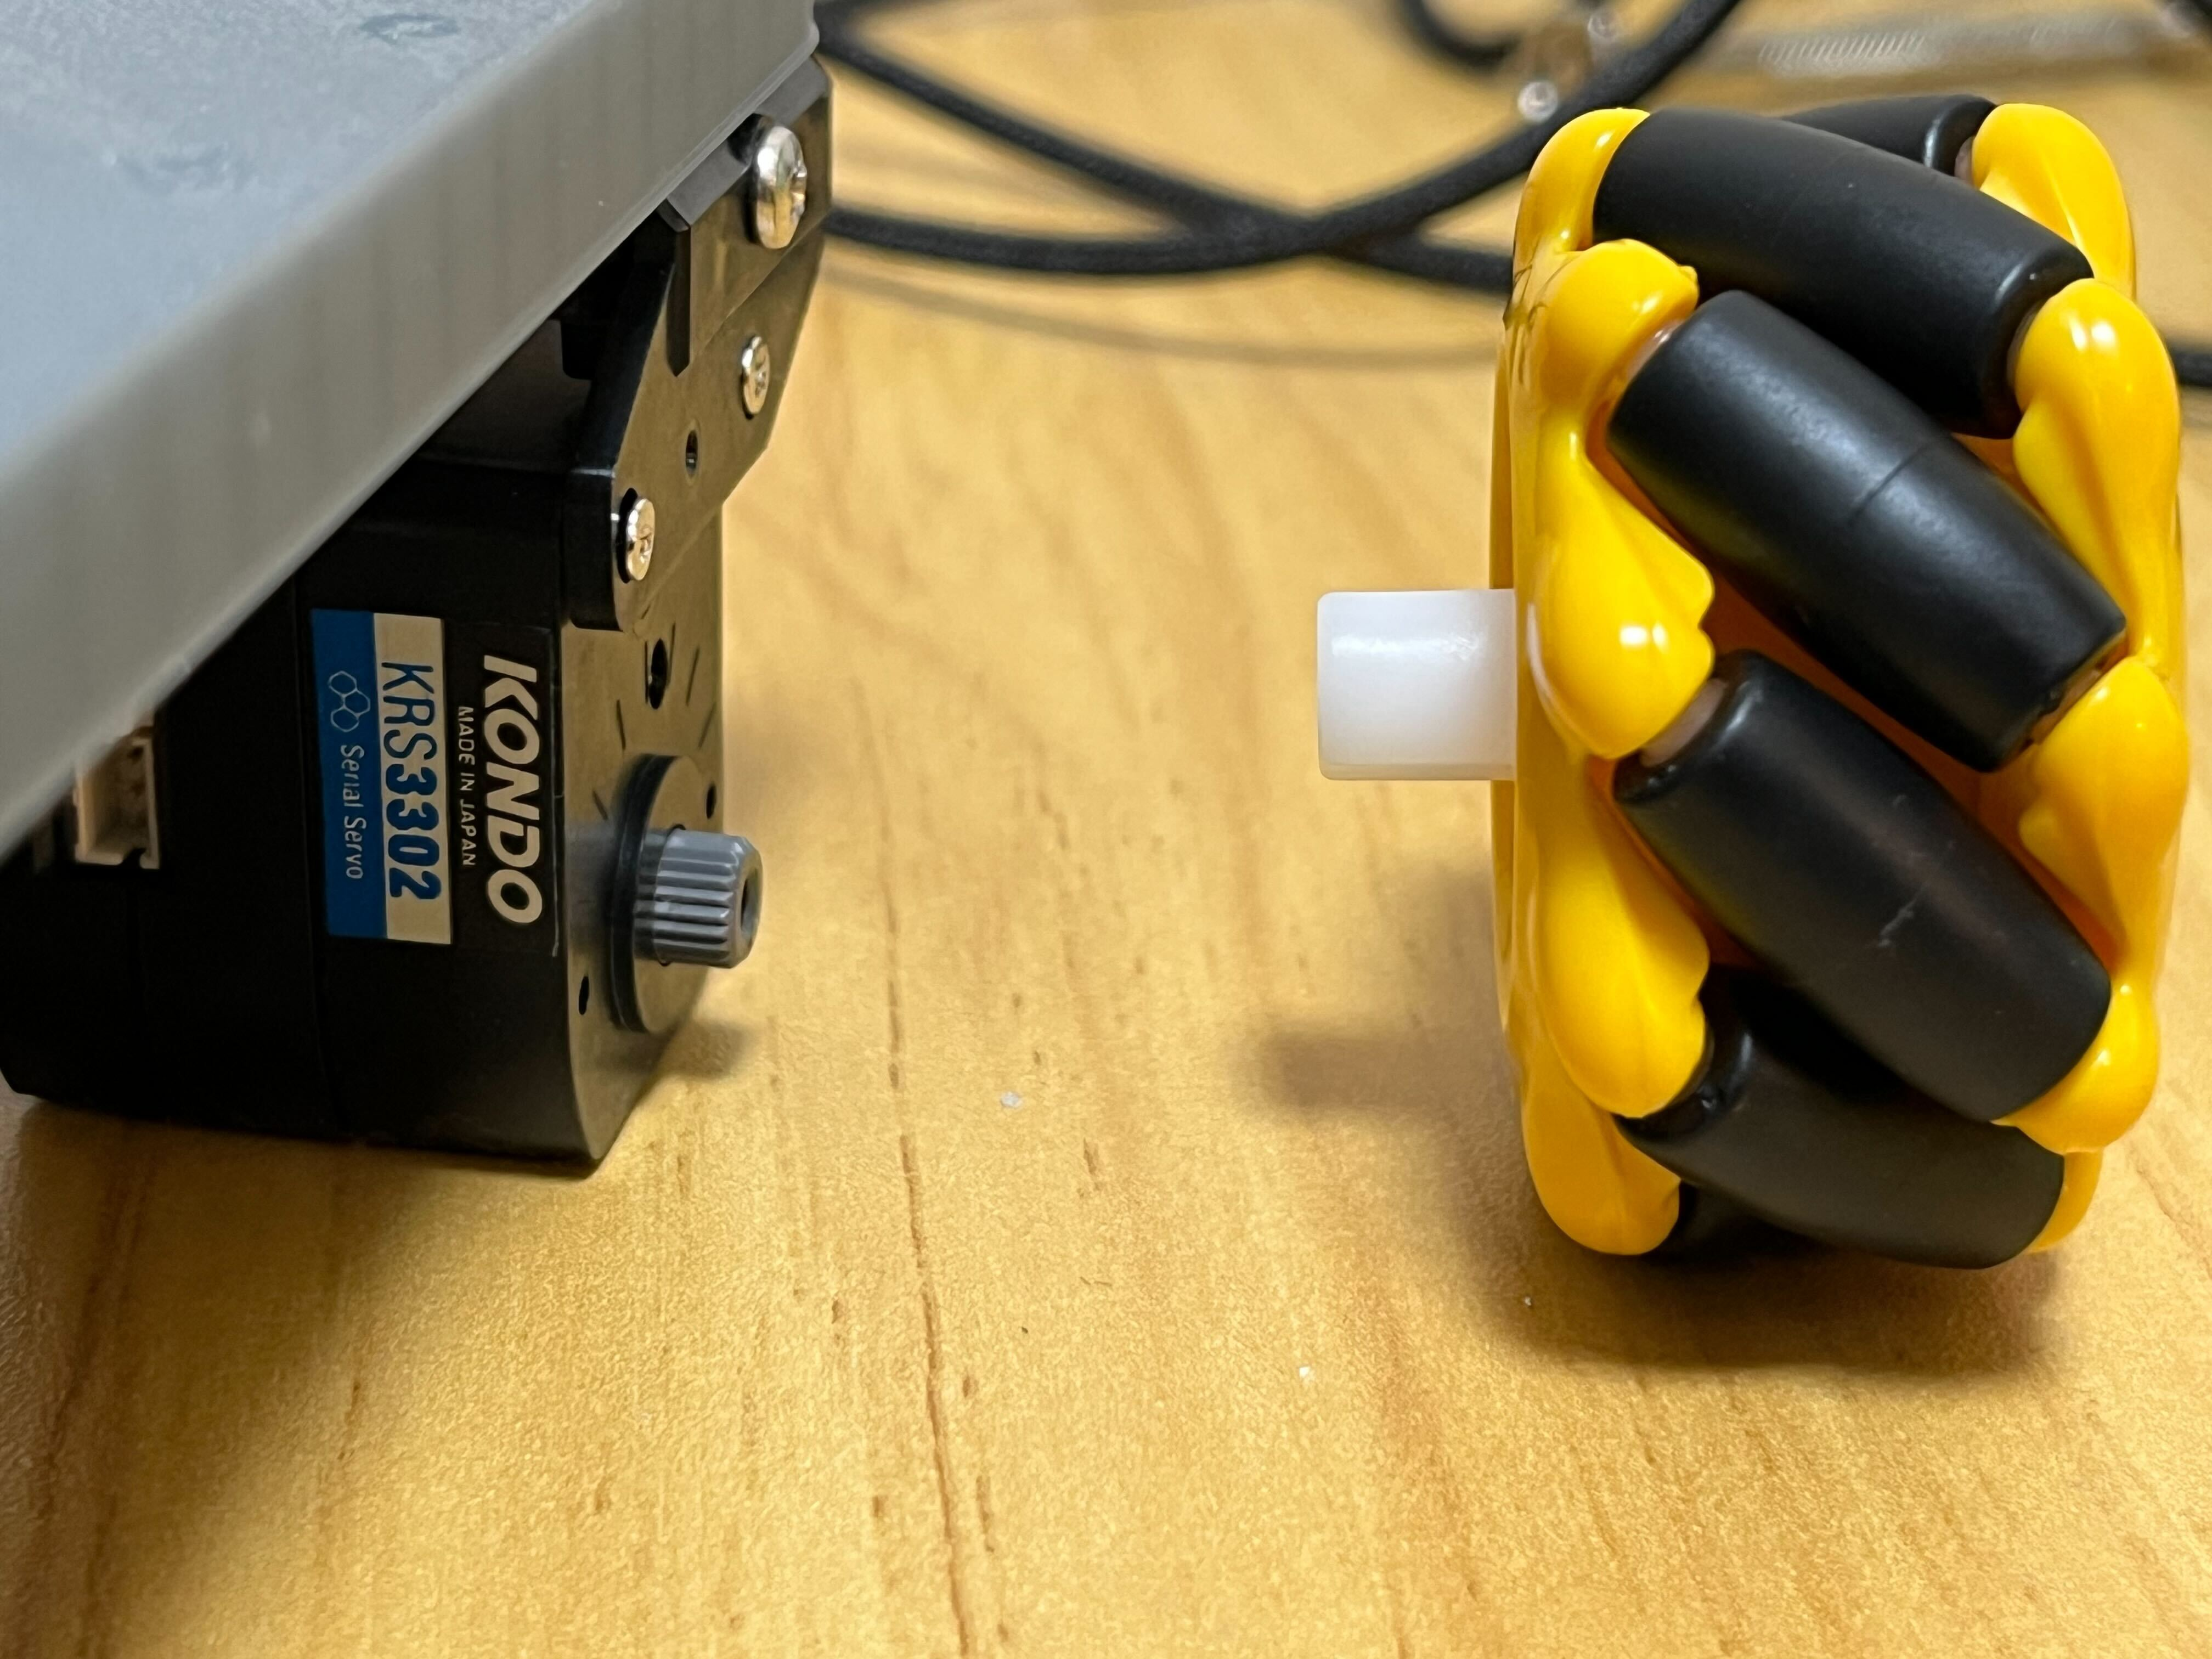
\includegraphics[width=\textwidth]{figures/body4.jpg}
      \caption{ベース板とホイールの接合部}
      \label{body4}
    \end{minipage}
  \end{figure}

  \subsection{ラケットの製作}
  当初は,運動量保存(卓球用語で言う「打撃のインパクト」)の観点から質量が大きいほうが良いと考え,本物のラケットを使おうと考えていた.しかし,サーボのトルクが小さいので,トルク負けして,シミュレーション通りのアームの軌道が実現できなかった.そこで,運動量保存云々行っている場合でなくなってしまったので,発表前々日に急遽プラスチックダンボールを購入し,カッターで切り出してラケットを自作した.ラバーは過去に自分が使っていたラケットに貼っていた使用済みのものを流用した.即席ラケットではありつつ,発表前日に卓球ショップに行ってラケット側面テープを購入し貼ることで,本物のラケットのような見た目にするなど工夫した.このようにラケットを変更したところ,ラケットを振る速さが速くなり,返球したボールの速さが目視で速くなった.

  \subsection{外装}
  当初の計画では,本プロジェクトはソフトウェアに注力し,ハードウェアはあまり凝らない予定だったが,「楽しめる/発表のときに楽しんでみてもらえる」ロボットを作るためには,ソフトだけではなく,外装も重要だと考えた.そこで,ユニフォーム,ゼッケンを製作した.また,靴,左腕,顔を製作し,内部のパーツを覆った.細かなこだわりとして,3Dプリンタでスポーツ選手らしい胸筋も製作した.また,3Dプリンタのフィラメントの色が様々だったのも,ペンキで黒に塗装し統一感を出した.図\ref{robot1}が外装前のロボットの様子で,図\ref{robot2}が外装後のロボットの様子である.
  \begin{figure}[H]
    \centering
    \begin{minipage}{0.48\textwidth}
      \centering
      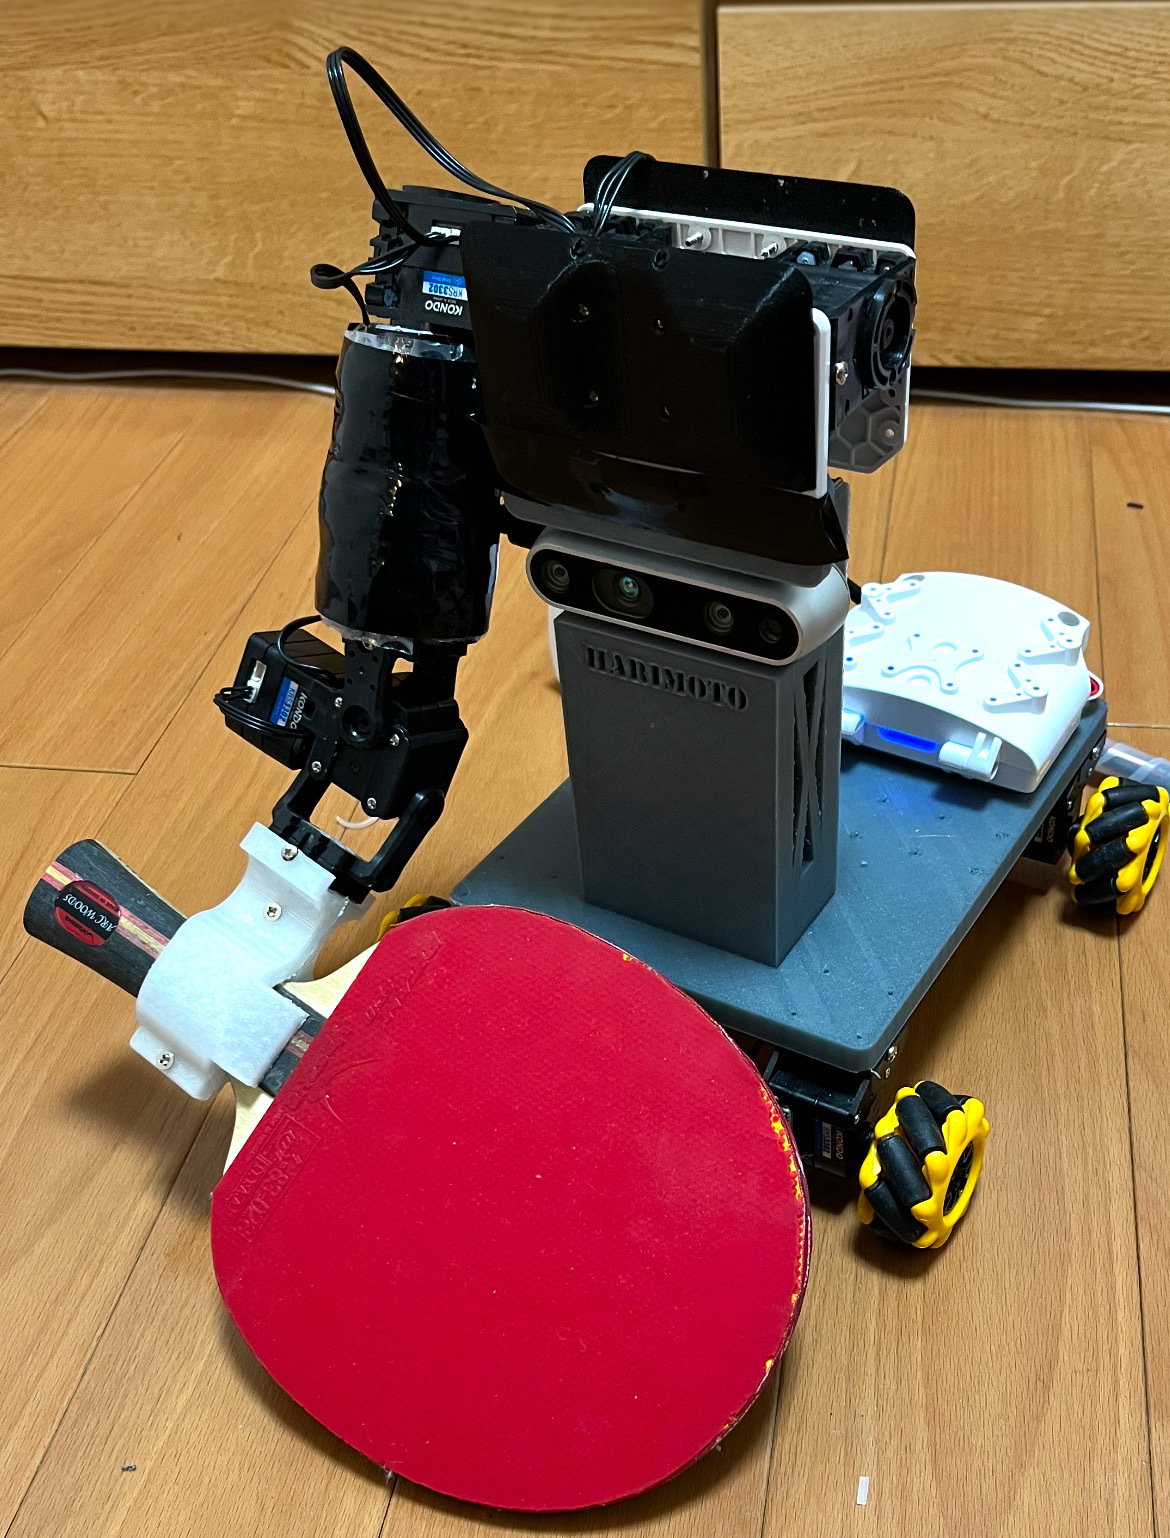
\includegraphics[width=\textwidth]{figures/robot1.jpg}
      \caption{外装前のロボット(ラケットは重い既成品)}
      \label{robot1}
    \end{minipage}
    \hfill
    \begin{minipage}{0.48\textwidth}
      \centering
      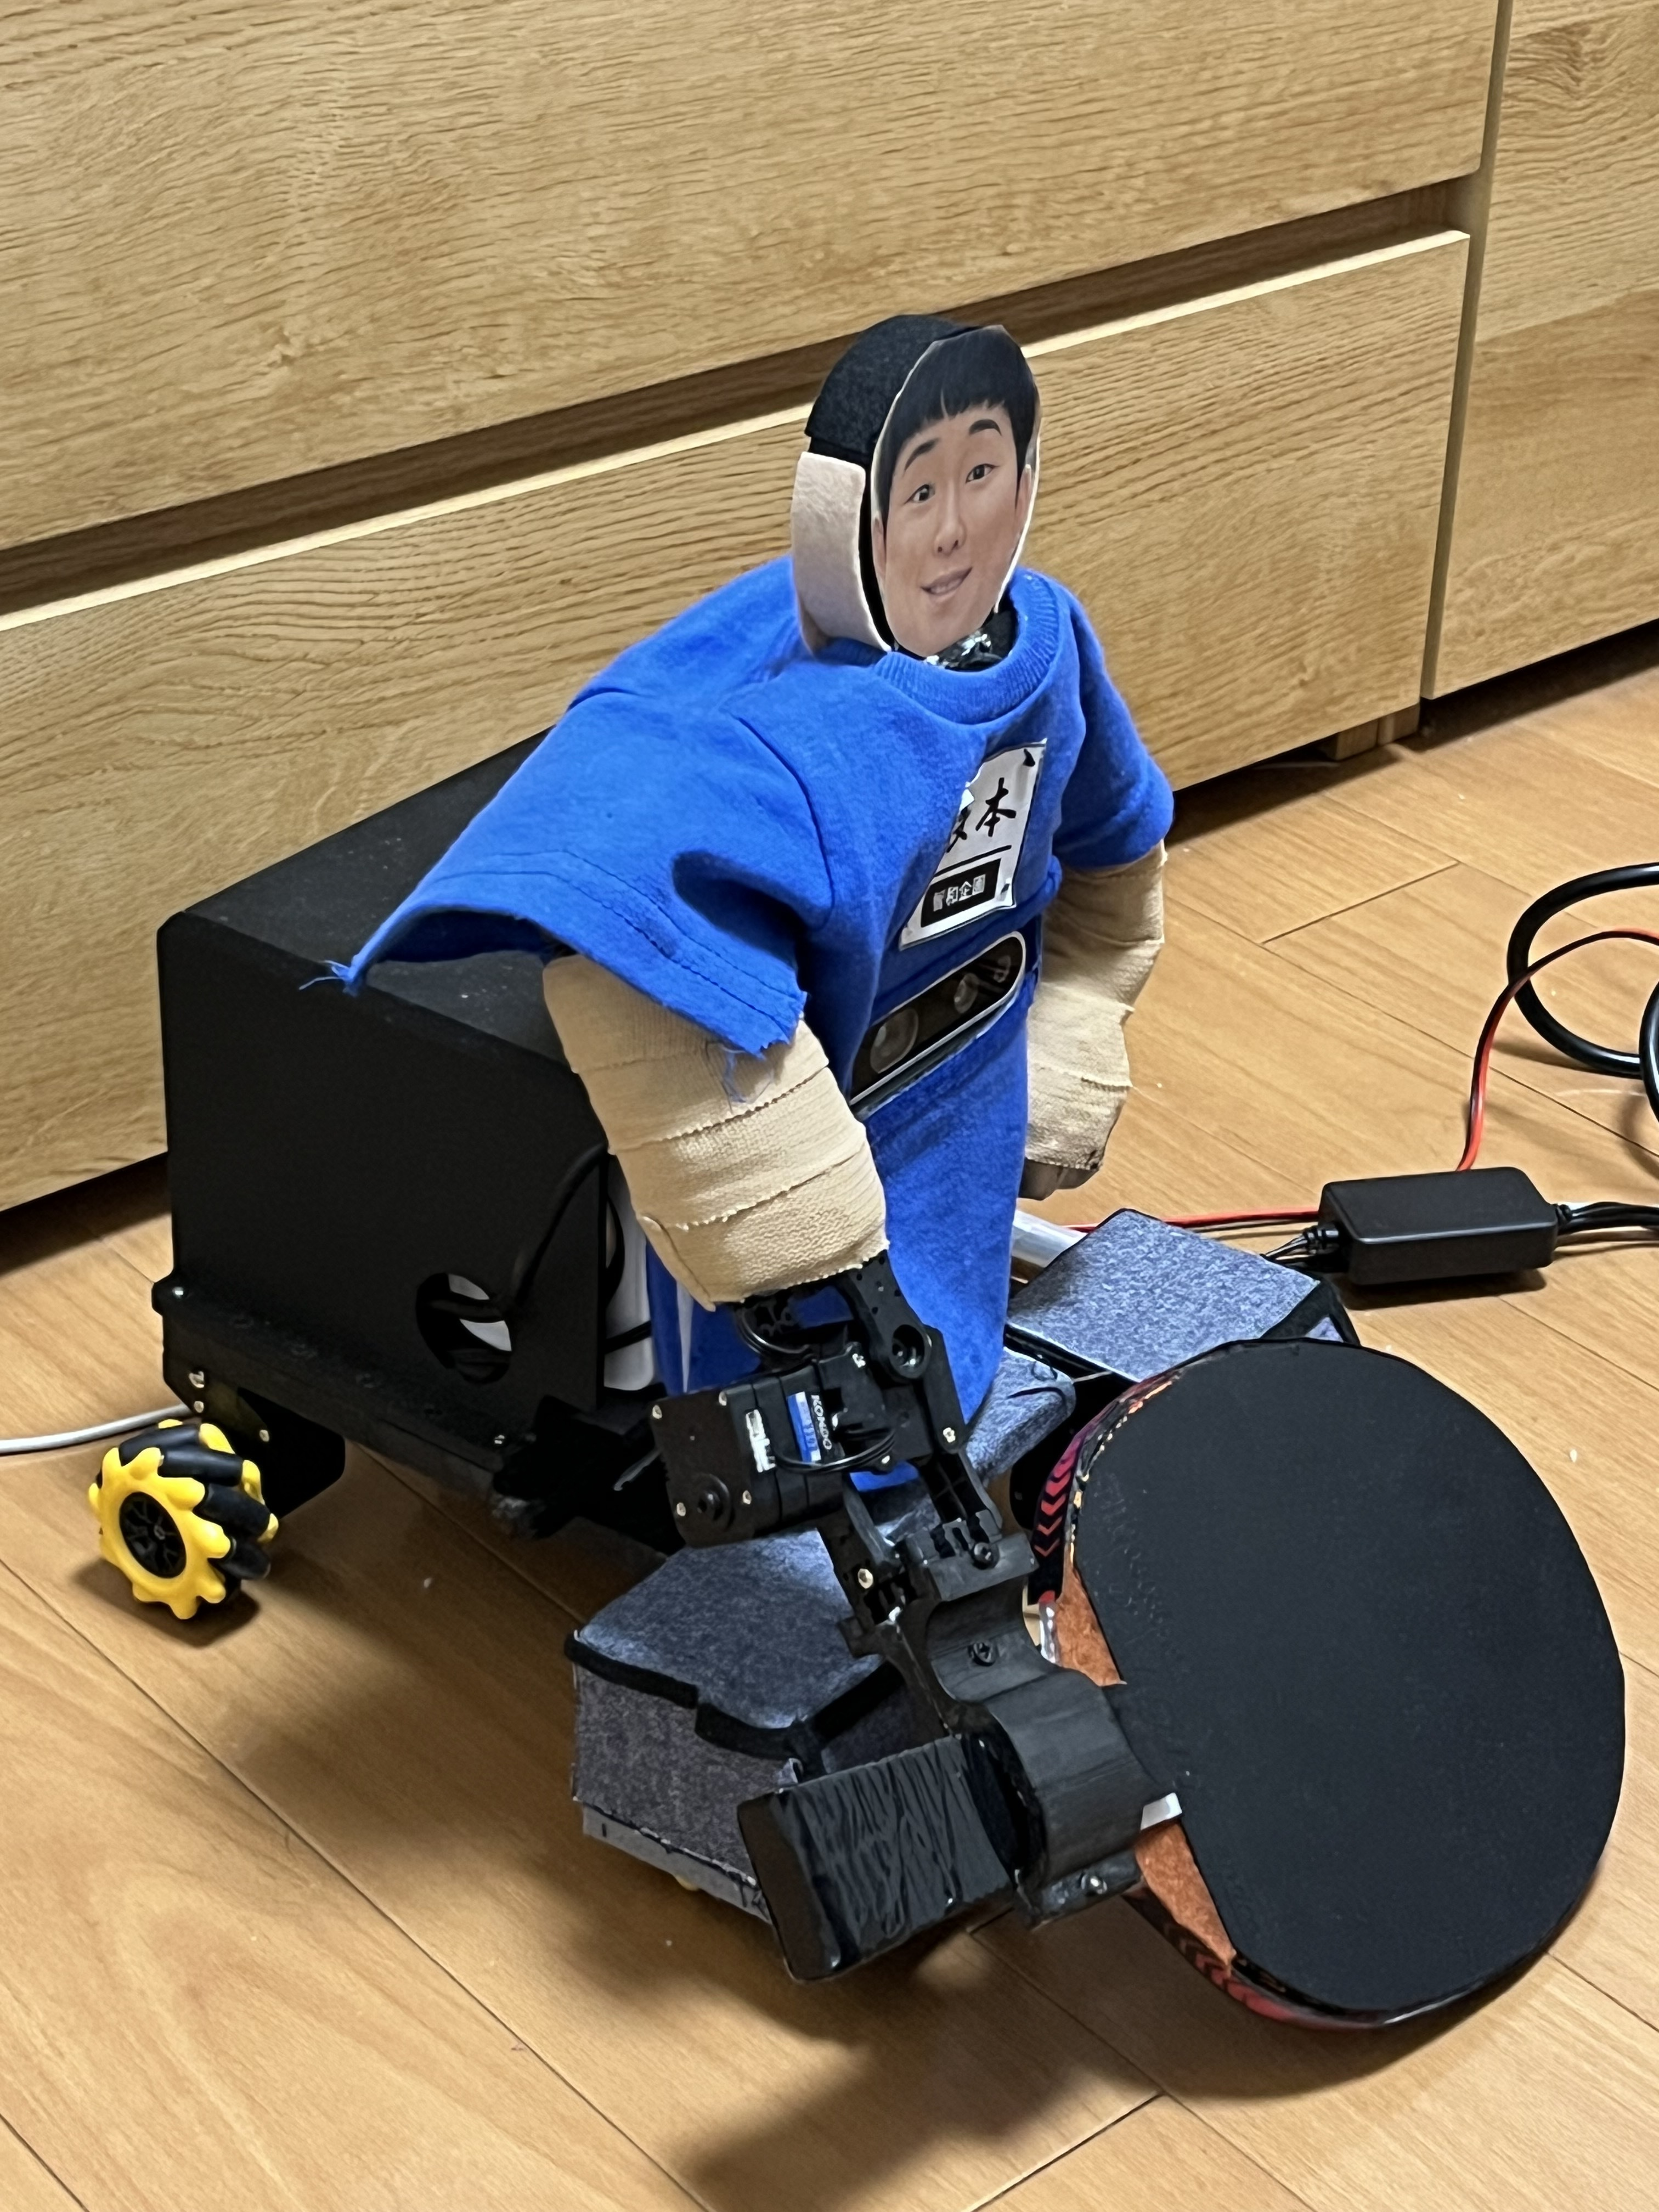
\includegraphics[width=\textwidth]{figures/robot2.jpg}
      \caption{外装後のロボット(ラケットは軽い自作品)}
      \label{robot2}
    \end{minipage}
  \end{figure}
\section{本プロジェクトを通した気づき(結論)}
ここまで述べてきたように,このロボットには,様々な苦労と工夫が詰まっているので,敢闘賞を頂けたのは嬉しいことだが,次章で述べるとおり,未だ課題も多い.

特に,本プロジェクトを行う前は,ボールの認識について「カメラの仕様的に大丈夫だろう」という甘い考えで望んでいたが,実際には,高速で移動する物体の認識がかなり難しいということを実感した(難しい分面白かったので問題ない).

\section{今後の展望}
  本プロジェクトを始めた当初の目標は,大きな目標として,
  \begin{enumerate}
    \item 来たボールを返球する
    \item ボールの着地予測地点に移動して返球する
    \item ボールの回転に応じて返球方法を動的に変えられるようにする
  \end{enumerate}
  の3点を掲げた.自主プロ発表会では,1.と2.を部分的ついて部分的に成功し発表することができた.一方で,
  \begin{enumerate}
    \item 返球できる確率は$\dfrac{1}{2}$程度に留まった
    \item 移動して対応できる距離はせいぜい$\pm 10 cm$であり,それ以上は返球が間に合わないため狭い範囲に留まった
    \item ドライブ打ちモードをコード上は実装したものの,動作パラメタのチューニングが間に合わなかった.また,プッシュ打ちとドライブ打ちを動的に変更するのは実現できなかった.
  \end{enumerate}
  は今後課題として残った.

  ロボットを五月祭に展示するにあたり,以下の課題について春休みに調査・開発を行うことにした.

  \subsection{画像認識:Depth情報のみからボールの位置を取得するアルゴリズムの開発}
  D435iを用いたボールの位置判定を行う際,Depth情報を使用する前にカラーフィルターを用いたマスク処理をしている.そのため,ColorとDepthの両方の情報を同時に取得する必要があり,この場合の取得周期は「60fps」が限界である(両者が同期する必要があるため).この制約が位置取得の遅れのボトルネックとなり,返球できる確率を制限していると考えられる.

  D435iは,Depth情報のみを使用する場合には300fpsを実現できるという公式の発表がある\cite{intel}.Depth情報だけを用いてボールの位置,速度,着地地点を予測するアルゴリズムを開発できれば,Color情報は不要となり,300fpsのフレーム情報を活用できるため,ラケットの振り遅れを大幅に減らし,返球確率を向上させることができると考えている.

  Depth情報を処理する際にクラスタリングを行うと処理速度が遅くなることを,このプロジェクトを通じて痛感したため,クラスタリングを経由しないアルゴリズムを考案する必要がある.

  以下は、本課題に対するアプローチで現時点で有用だと考えられるアプローチ(仮説)である.

  \begin{itemize}
    \item 深尾教授のロボットコントロールの講義で学んだ自動運転における「時間的に連続するフレームの差分を取ることで移動する障害物(人など)の情報を抽出する」手法を応用することで,移動物体であるボールを効率的に検出できるのではないかと考えている.時間計算量は処理で扱う点数(特徴点の数)に依存するため,この特徴点抽出により処理全体が高速化できると予想している.

    \item 國吉教授のロボットインテリジェンスの講義で学んだ「Time to Collision(衝突までの時間)」の概念を用いることで,ボールの着地予測時間を簡単に算出でき,計算処理の高速化が期待できる.

    \item 矢野倉先生から助言をいただいた「半円殻(卓球ボールの像)」のマッチングや,岡田ゼミで使用した「Hough変換による円抽出」を3次元空間に応用する方法(射影処理など)を通じて,ボールを抽出する手法を取り入れたいと考えている.
  \end{itemize}

  この春休みを通じて,上記の仮説を検証し,計算量を削減するための特徴点抽出とDepthフレームからの卓球ボール高速検出の課題に取り組んでいく.

  \subsection{ドライブ打ちモードのパラメタチューニング}
  前述したとおり,ドライブモードをできるシステム構成は完成しているので,ロボットアームの初期姿勢やラケットを振るアームの速度・経路を調整する.また,ボールがこの範囲に着地するときにラケットを振るという基準値もプッシュ打ちモードとは異なるはずなので,その範囲(スイートスポットの値など)も調整する.

\section{謝辞}
本プロジェクトに取り組むに際し,ラフスケッチ・詳細スケッチに対して実現可能性や計画性,機構面で改善すべき点についてアドバイスをくださった小島邦生先生,Depth Cameraによる画像処理の方法やKXRのConfigurationについての逐次の質問やロボットパーツなどの資材の貸出対応で大変お世話になった矢野倉伊織先生,3Dプリンタ環境をご提供くださったメカノデザイン工房の技術職員の方々,アドバイスをくれた機械情報工学科の同級生に御礼申し上げます.


\begin{thebibliography}{7}
  \bibitem{omron}
  八瀬哲志. (2020). 卓球ロボットFORPHEUS. 日本ロボット学会誌, Vol.38(No.4), pp.318-322. \url{https://www.jstage.jst.go.jp/article/jrsj/38/4/38_38_318/_pdf}
  \bibitem{detect1}
  iory, ``color\_filter.launch,'' GitHub Gist. [Online]. Available: 
  \url{https://gist.github.com/iory/c0b13faa5bceb062dcc37376a7af9f1b}
  \bibitem{detect2} 
  Michi-Tsubaki, ``recognize\_wound.launch,'' jsk\_demosm GitHub. [Online]. Available: 
  \url{https://github.com/Michi-Tsubaki/jsk_demos/blob/jsk_2024_10_semi/jsk_2024_10_semi/pr2_surgery/launch/recognize_wound.launch}
  \bibitem{detect3}
  porizou1, ''ubuntu20.04とROS NoeticでRealSenseを使う手順'' Qiita. [Online]. Available: 
  \url{https://qiita.com/porizou1/items/be1eb78015828d43f9fb}
  \bibitem{mecanum} 
  iory, ``[jedy\_bringup] support mecanum drive using ridgeback\_control \#2,'' robot-programming, GitHub. [Online]. Available: 
  \url{https://github.com/iory/robot-programming/pull/2}

  \bibitem{sound} 
  jsk-ros-pkg, ``speak.l,'' jsk\_pr2eus, GitHub. [Online]. Available: 
  \url{https://github.com/jsk-ros-pkg/jsk_pr2eus/blob/master/pr2eus/speak.l}

  \bibitem{intel}
  intel realsense, ''High Speed Capture for Intel® RealSense™ Depth Cameras'', April 8, 2020,
  \url{https://www.intelrealsense.com/high-speed-mode-at-300-fps-for-depth-camera/}
\end{thebibliography}

\dotfill

\section{(参考)環境構築・実行方法(Github)}
  本プロジェクトに関する全てのソースコードと自作パーツのモデルは, \url{https://github.com/Michi-Tsubaki/ping-pong-robot}で公開している.ソースコードについてはそこを参照してほしい.また,ロボットのURDFを作成しているため,実機がなくても手元の環境で誰でもシミュレーション可能である.
  \subsection{環境構築}
  知能ロボット行動プログラミングの演習を受講後の学科PCの環境(ubuntu20.04, ros noetic)で開発を行った.以下を実行し,リポジトリをホームディレクトリにクローンする.
  \begin{screen}
    cd ~ \\
    git clone https://github.com/Michi-Tsubaki/ping-pong-robot.git \\
    cd ~/ping-pong-robot
  \end{screen}
  \subsection{実行方法}
  ターミナルを開いて,以下を実行し,
  \begin{screen}
    cd ~/ping-pong-robot \\
    source devel/setup.bash \\
    roslaunch HARIMOTO all.launch \#画像処理やアームコントローラのノードを起動
  \end{screen}
  また,別のターミナルで
  \begin{screen}
    cd ~/ping-pong-robot\\
    source devel/setup.bash \\
    roscd HARIMOTO/src \\
    emacs -nw main.l \\
    M+x shell RET\\
    roseus \\
    load "main.l"
  \end{screen}
  を実行することでロボットのメインプログラムを動かすことができる.

  build済みの環境をcloneすることになる.エラーが出る場合は,パスがおかしかったり,必要なros packageが存在しない可能性がある.この場合,sudo apt updateやrosdep installを実行する必要がある.その後,catkin buildをやり直す(clean buildがよい).
\end{document}